%%%%%%%%%%%%%%%%%%%%%%%%%%%%%%%%%%%%%%%%%
% Masters/Doctoral Thesis 
% LaTeX Template
% Version 1.43 (17/5/14)
%
% This template has been downloaded from:
% http://www.LaTeXTemplates.com
%
% Original authors:
% Steven Gunn 
% http://users.ecs.soton.ac.uk/srg/softwaretools/document/templates/
% and
% Sunil Patel
% http://www.sunilpatel.co.uk/thesis-template/
%
% License:
% CC BY-NC-SA 3.0 (http://creativecommons.org/licenses/by-nc-sa/3.0/)
%
% Note:
% Make sure to edit document variables in the Thesis.cls file
%
%%%%%%%%%%%%%%%%%%%%%%%%%%%%%%%%%%%%%%%%%

%----------------------------------------------------------------------------------------
%	PACKAGES AND OTHER DOCUMENT CONFIGURATIONS
%----------------------------------------------------------------------------------------

\documentclass[11pt, oneside]{Thesis} % The default font size and one-sided printing (no margin offsets)

\graphicspath{{Figures/}} % Specifies the directory where pictures are stored

\usepackage{algorithm}
\usepackage[]{algorithmic}
\usepackage{subfig}
\usepackage{graphicx}
%\usepackage{subfigure}
\usepackage{Missing_Packages/multiFloats}
\usepackage{url}
\usepackage{wrapfig}
\usepackage{float}
\usepackage[flushleft]{threeparttable}
\usepackage{url}
\usepackage{color}
%\usepackage{pslatex}
%\usepackage{natbib}
\usepackage{paralist}
\usepackage{comment}
\usepackage{tablefootnote}
%\usepackage{flushend}
%\renewcommand{\algorithmiccomment}[1]{// #1}
%\renewcommand{\bibfont}{\small}
%\renewcommand{\bibsep}{0.05cm}
\input{abreviations}

\usepackage[square, numbers, comma, sort&compress]{natbib} % Use the natbib reference package - read up on this to edit the reference style; if you want text (e.g. Smith et al., 2012) for the in-text references (instead of numbers), remove 'numbers' 
\hypersetup{urlcolor=black, colorlinks=true} % Colors hyperlinks in blue - change to black if annoying
\title{\ttitle} % Defines the thesis title - don't touch this

\begin{document}

%\frontmatter % Use roman page numbering style (i, ii, iii, iv...) for the pre-content pages

\setstretch{1.3} % Line spacing of 1.3

% Define the page headers using the FancyHdr package and set up for one-sided printing
\fancyhead{} % Clears all page headers and footers
\rhead{\thepage} % Sets the right side header to show the page number
\lhead{} % Clears the left side page header

%\pagestyle{fancy} % Finally, use the "fancy" page style to implement the FancyHdr headers

\newcommand{\HRule}{\rule{\linewidth}{0.5mm}} % New command to make the lines in the title page

% PDF meta-data
\hypersetup{pdftitle={\ttitle}}
\hypersetup{pdfsubject=\subjectname}
\hypersetup{pdfauthor=\authornames}
\hypersetup{pdfkeywords=\keywordnames}

%----------------------------------------------------------------------------------------
%	TITLE PAGE
%----------------------------------------------------------------------------------------
\setcounter{page}{1}
\thispagestyle{empty}
%\begin{titlepage}
\begin{center}

%\textsc{\LARGE \univname}\\[1.5cm] % University name
%\textsc{\Large Doctoral Thesis}\\[0.5cm] % Thesis type
%\HRule \\[0.4cm] % Horizontal line
\vspace*{5cm}
{\huge \bfseries \ttitle}\\[0.4cm] % Thesis title
%\HRule \\[1.5cm] % Horizontal line

%\begin{minipage}{0.4\textwidth}
\textsc{\authornames}
%\end{minipage}\\[3cm]

%{\large \today}\\[4cm] % Date
\vfill

\end{center}
%\end{titlepage}

%-----------------------------------------------------------------------------
% 2nd page is empty
%-----------------------------------------------------------------------------
\clearpage
\pagestyle{fancy}
\null
\newpage

%-----------------------------------------------------------------------------
% 3rd page: title + default dutch text
%-----------------------------------------------------------------------------
\pagestyle{fancy}
\begin{center}

%%%\begin{center}
\vspace*{3cm}
{\huge\bf Holistic Indexing}\\
%\vspace*{0.5cm}
%{\huge\bf Column-Stores}\\
%%%\end{center}

\vspace*{3cm}

{\sc Academisch Proefschrift}

\vspace{1cm}
ter verkrijging van de graad van doctor\\
aan de Universiteit van Amsterdam,\\
op gezag van de Rector Magnificus\\
prof. ... \\
ten overstaan van een door het\\ 
college voor promoties ingestelde commissie\\
in het openbaar te verdedigen\\
in ... \\
op ...

\vspace*{3cm}

door\\
Eleni Petraki\\
geboren te Karditsa, Griekenland\\
\end{center}
\clearpage

%----------------------------------------------------------------------------------------
%	Promotiecommissie
%----------------------------------------------------------------------------------------
\pagestyle{fancy}
\noindent
\begin{tabular}{ll}
\textbf{Promotiecommissie}  & \\
	   & \\
Promotor:  & Prof. dr. M.L. Kersten\\
           & \\
Copromotor:& Prof. dr. S. Manegold\\
	   & Asst. Prof. dr. S. Idreos\\
           & \\
Overige Leden: & Prof. dr. ... \\
           & Prof. dr. ... \\
           & Prof. dr. ... \\
           & Prof. dr. ... \\
           & Prof. dr. ... \\
\end{tabular}
\\
\\
\\
\noindent
Faculteit der Natuurwetenschapen, Wiskunde en Informatica
\clearpage 

%----------------------------------------------------------------------------------------
%	CWI, MonetDB, SIKS
%----------------------------------------------------------------------------------------
\pagestyle{fancy} % No headers or footers for the following pages

\includegraphics[width=1.7cm]{Figures/CWIlogo}
\\
\\
{The research reported in this thesis has been partially carried out at CWI,
the Dutch National Research Laboratory for Mathematics 
and Computer Science, within the theme Database Architectures and Information Access, 
a subdivision of the research cluster Information Systems.}
\\
\\
\\
\includegraphics[width=1.7cm]{Figures/monetdb_logo}
\\
\\
{The research reported in this thesis has been partially carried out as part of the continuous research and development of the MonetDB
open-source database management system.}
\\
\\
\\
\includegraphics[width=1.7cm]{Figures/siks_logo.eps}
\\
\\
{SIKS Dissertation Series No-nnnn-nn.\\
The research reported in this thesis has been carried out under the auspices 
of SIKS, the Dutch Research School for Information and Knowledge Systems.}
\\
\\
\\
ISBN nn nnnn nnn n
\clearpage 

%----------------------------------------------------------------------------------------
%	DEDICATION
%----------------------------------------------------------------------------------------

\pagestyle{empty} % Page style needs to be empty for this page
%\setstretch{1.3} % Return the line spacing back to 1.3
%\dedicatory{For/Dedicated to/To my\ldots} % Dedication text
\dedicatory{Dedicated to my parents, Sofia and Theodoros,\newline
	   and my husband, Evangelos.} % Dedication text
\clearpage % Start a new page

%----------------------------------------------------------------------------------------
%	QUOTATION PAGE
%----------------------------------------------------------------------------------------

\pagestyle{empty} % No headers or footers for the following pages

\null\vfill % Add some space to move the quote down the page a bit

\textit{``The time will come when diligent research over long periods will bring to light things which now lie hidden. A single lifetime, even though entirely devoted to the sky, would not be enough for the investigation of so vast a subject... And so this knowledge will be unfolded only through long successive ages. There will come a time when our descendants will be amazed that we did not know things that are so plain to them... Many discoveries are reserved for ages still to come, when memory of us will have been effaced."}

\begin{flushright}
Seneca, Natural Questions 
\end{flushright}

\vfill\vfill\vfill\vfill\vfill\vfill\null % Add some space at the bottom to position the quote just right

\clearpage % Start a new page

%----------------------------------------------------------------------------------------
%	LIST OF CONTENTS
%----------------------------------------------------------------------------------------

\pagestyle{fancy} % The page style headers have been "empty" all this time, now use the "fancy" headers as defined before to bring them back

\lhead{\emph{Contents}} % Set the left side page header to "Contents"
\tableofcontents % Write out the Table of Contents
\clearpage % Start a new page



%----------------------------------------------------------------------------------------
%	THESIS CONTENT - CHAPTERS
%----------------------------------------------------------------------------------------

%\mainmatter % Begin numeric (1,2,3...) page numbering

\pagestyle{fancy} % Return the page headers back to the "fancy" style
% Include the chapters of the thesis as separate files from the Chapters folder
% Uncomment the lines as you write the chapters

\section{Introduction}
\label{sec:intro}

\begin{table*}
\begin{center}

\begin{tabular}{ccccccc}
\hline
\cline{1-7}
Indexing& Statistical&Exploitation of idle resources & Exploitation of idle resources & Index  		 & Updates, & Workload\\
        & analysis   & \emph{before} query processing& \emph{during} query processing & materialization  & projection cost &\\
\hline
Offline & $\surd$ & $\surd$ & $\times$  & full & high & static \\ 
Online & $\surd$ & $\times$ & $\surd$  & full & high & dynamic\\
Adaptive & $\times$ & $\times$ & $\times$  & partial & low & dynamic\\
Holistic & $\surd$ & $\surd$ & $\surd$  & partial & low & dynamic\\
\hline
\label{tab:qualitative}
\end{tabular}
\vspace{-0.45cm}
 \caption{Qualitative difference among offline, online, adaptive and holistic indexing.}
\vspace{-0.7cm}
\end{center}
\end{table*}

The big data era is causing the research community to rethink fundamental issues 
in the design of database systems  
towards more usable systems \cite{UsableDatabases} that can access data better and faster 
%\cite{blinkdb,MAD,shark,exploration,hinge, hazy,earl,GuidedInteraction, RequirementsSciDB, datacuration,energypartitioning},
\cite{exploration,hinge, hazy,earl},
 that can better exploit modern hardware and opportunities for massive parallelization
%\cite{swissbox,elastras,hadoop+,cod,dbseer},
\cite{hadoop+}
 that can support efficient processing of OLTP and/or OLAP queries
% \cite{nodb,shareddb,hstore,hyper,bitweaving}
 \cite{nodb,hstore,hyper,bitweaving}.
% or even exploit crowdsourcing for query processing \cite{crowdq,crowddb}.

\textbf{The Physical Design Problem.} 
Physical design, and in particular proper index selection, is a predominant factor for the performance of database systems and has only become more crucial in the big data era.
With new dynamic and exploratory environments, physical design becomes especially hard given the instability of workloads and the continuous stream of big data; a single physical design choice is not necessarily correct or useful for long stretches of time, while at the same time workload knowledge is scarce given the exploratory user behavior.

\textbf{State-of-the-Art.} In database applications, where ``the future is known'', physical design is assigned to database administrators
who may also be assisted by auto-tuning tools 
\cite{DBLP:conf/vldb/AgrawalCKMNS04,DBLP:conf/vldb/DagevilleDDYZZ04,DBLP:conf/vldb/ZilioRLLSGF04}.
Still though, a significant amount of human intervention is necessary and everything needs to happen offline.
Thus, offline indexing can be applied with good results only on applications where there is enough workload 
knowledge and idle time to prepare the physical design appropriately before queries arrive.

Unfortunately, for many modern applications ``the future is unknown'', e.g., in scientific databases, social networks, web logs, etc.
In particular, the query processing patterns follow an exploratory behavior, which changes so arbitrarily that it cannot be predicted.
Such environments cannot be handled by offline indexing.
Online indexing \cite{DBLP:conf/icde/BrunoC07,DBLP:conf/sigmod/SchnaitterAMP06} 
and adaptive indexing \cite{DBLP:conf/cidr/IdreosKM07} 
are two approaches to automatic physical design in such dynamic environments, but none of them in isolation handles the problem sufficiently.
Online indexing periodically refines the physical design but it may negatively affect running queries every time
it needs to use resources for reconsidering the physical design and it may not be quick to follow the workload changes as it reacts only periodically. 
Adaptive indexing does not have this problem as it introduces continuous, incremental and partial index refinement 
but it adjusts the physical design only during query processing based on queries.

\textbf{Always Indexing.}
In this paper, we make the observation that in real systems there are plenty of resources that remain under-utilized and 
we propose to exploit those resources to be able to better address dynamic and  ad-hoc environments. 
In particular, we focus on exploiting CPU cycles to the maximum by continuously detecting idle CPU cycles
and using them to refine the physical design (in parallel with query processing).
Such idle CPU cycles occur when the system  does not exploit all available cores up to 100\%.
% (non-peak workload).
%i.e., either because the workload is not enough to saturate the CPUs or because the current tasks performed for 
%query processing are not easy to parallelize to the point where all available CPU power can be  exploited
%or when there are no active user queries (\emph{idle time}).
We distinguish between ``\emph{idle time}'' as in
``\emph{there is no user-driven workload at all and the entire CPU (all its hardware contexts) is idle (except possible occasional operating system background activity)}''
and ``\emph{idle CPU resources}'' as in
``\emph{the active user-driven workload does / can not use all physically available CPU hardware contexts.}'' 
Intuitively, there are two options when resources are under-utilized but still there are active queries in the system.
The first option is to introduce more parallel query processing algorithms to maximize utilization for the existing workload. The second one is to exploit the extra resources towards a different goal (extra indexing actions in our case). We investigate and compare both directions.


%\begin{figure}[t]
%\begin{center}
%\includegraphics[trim=4cm 22cm 12cm 2.8cm]{qualitative}
%\caption{Indexing Approaches.}
%\vspace{-0.4 in}
%\label{fig:various}
%\end{center}
%\end{figure}

\textbf{Holistic Indexing.} In this paper, we introduce a new indexing approach, 
called \emph{holistic indexing}.
Holistic indexing  addresses the automatic physical design problem in 
modern applications with  dynamic and exploratory workloads.
%\textcolor{red}{where there is no prior knowledge about how many under-utilized CPU resources will be available}.  
It continuously monitors the workload and the CPU utilization; 
when idle CPU cycles are detected, holistic indexing exploits them in order to partially and incrementally 
adjust the physical design based on the collected statistical information.
Each index refinement step may take only a few microseconds to complete and the system will typically perform
several such steps in one go depending on available system resources.
Everything happens in parallel to query processing but without disturbing running queries.
The net effect is that holistic indexing refines the physical design,
% there are more chances for future queries to enjoy better  data access patterns.
improving performance and robustness by enabling better data access patterns for future queries.
Table~\ref{tab:qualitative} summarizes the qualitative difference between holistic indexing and current state-of-the-art indexing approaches.
Compared to past approaches, holistic indexing manages to minimize both initialization and maintenance costs, 
as it relies on partial indexing, and to exploit all possible CPU resources
%before and/or during query processing, 
in order to provide a more complete physical design.

\textbf{Contributions.}
Our contributions are as follows:
\vspace{-0.5em}
\begin{itemize}
  \setlength{\itemsep}{0pt}
  \setlength{\parskip}{0pt}
  \setlength{\parsep}{0pt}
\item We introduce the idea of exploiting idle CPU resources towards 
continuously adapting the physical design to ad-hoc and dynamic workloads.
\item We discuss  in detail the design of holistic indexing on top of modern column-store architectures, i.e.,
how to detect and exploit idle CPU resources during query processing.
\item We implemented holistic indexing in  an open-source column-store, MonetDB \cite{DBLP:journals/debu/IdreosGNMMK12, monetdb}.
%\textcolor{red}{The code is publicly available in \cite{holindex}.} 
Through a detailed experimental analysis both with microbenchmarks and with TPC-H 
we demonstrate that we can exploit idle CPU resources to prepare the physical design better,
leading to significant improvements over past indexing approaches in dynamic environments. 
\end{itemize}
\vspace{-0.5em}

\textbf{Paper Structure.} The rest of the paper is structured as follows:
Section~\ref{sec:relwork} provides an overview of related work.
In Section~\ref{sec:background}, we shortly recap the basics of column-store architectures 
and the basics of adaptive indexing.
Then, Section~\ref{sec:problem} introduces holistic indexing, while Section~\ref{sec:experiments} presents a detailed experimental analysis.
Finally, Section~\ref{sec:conclusions} discusses future work and concludes the paper. 


 
%\addcontentsline{toc}{chapter}{}
\clearpage

\chapter{Related Work and Background} % Main chapter title

\label{RelatedWork} % For referencing the chapter elsewhere, use \ref{Chapter1} 

\lhead{Chapter 2. \emph{Related Work and Background}} % This is for the header on each page - perhaps a shortened title

%----------------------------------------------------------------------------------------
%	SECTION 1
%----------------------------------------------------------------------------------------

Intro

%----------------------------------------------------------------------------------------
%	SECTION 1
%----------------------------------------------------------------------------------------

\section{Row-oriented Storage and Data Access}
\label{sec:row-oriented}

%----------------------------------------------------------------------------------------
%	SECTION 1
%----------------------------------------------------------------------------------------

\section{Column-stores}
\label{sec:column-stores}

%----------------------------------------------------------------------------------------
%	SECTION 1
%----------------------------------------------------------------------------------------

\section{Indices}
\label{sec:indices}

%----------------------------------------------------------------------------------------
%	SECTION 1
%----------------------------------------------------------------------------------------

\section{Offline Indexing}
\label{sec:holistic}

Offline indexing is the earliest approach on self-tuning database systems.
Nowadays, all major database products offer auto-tuning tools \cite{DBLP:conf/vldb/AgrawalCKMNS04,DBLP:conf/vldb/DagevilleDDYZZ04, DBLP:conf/vldb/ZilioRLLSGF04} to automate the database physical design.
Auto-tuning tools mainly rely on a ``what-if analysis'' \cite{DBLP:conf/sigmod/ChaudhuriN98} and close interaction with the optimizer \cite{DBLP:conf/vldb/ChaudhuriN97} to decide which indices are potentially more useful for a given workload.

Offline indexing  requires heavy involvement of a database administrator (DBA).
Specifically, a DBA invokes the tool and provides its input, i.e., a representative workload.
The tool analyzes the given workload and recommends an appropriate physical design.
However, the DBA is the one that decides which of the changes in the physical design should be applied.
The main limitation of offline indexing appears when the workload cannot be predicted and/or there is not enough idle time to invest in the offline analysis and the physical design implementation. 


%----------------------------------------------------------------------------------------
%	SECTION 1
%----------------------------------------------------------------------------------------

\section{Online Indexing}
\label{sec:online}

Online indexing addresses the limitation of offline indexing.
Instead of making all decisions a priori, the system continuously monitors the workload and the physical design is periodically reevaluated.
System COLT \cite{DBLP:conf/sigmod/SchnaitterAMP06} was one of the first online indexing approaches.
COLT continuously monitors the workload and periodically in specific epochs, i.e., every N queries, it reconsiders the physical design.
The recommended physical design might demand creation of new indices or dropping of old ones.
COLT requires many calls to the optimizer to obtain cost estimations.
A ``lighter'' approach, i.e., requiring less calls to the optimizer, was proposed later \cite{DBLP:conf/icde/BrunoC07}.
Soft indices \cite{DBLP:conf/icde/LuhringSSS07} extended the previous 
online approaches by building full indices on-the-fly concurrently with queries on the same data, sharing the scan operator.

The main limitation of online indexing is that reorganization  of the physical design can be a costly action
that a) requires a significant amount of time to complete and b) requires a lot of resources.
This means that online indexing is appropriate mainly for moderately dynamic workloads where the query patterns do not change
very frequently. Otherwise, it may be that by the time we finish adapting the physical design, the workload has changed again
leading to a suboptimal performance.


%----------------------------------------------------------------------------------------
%	SECTION 1
%----------------------------------------------------------------------------------------

\section{Adaptive Indexing}
\label{sec:cracking}


Adaptive indexing is the latest and the most lightweight approach in self-tuning databases.
Adaptive indexing  addresses the limitations of offline and online indexing for dynamic workloads; 
it  instantly adjusts to workload changes by building or refining indices partially and incrementally as part of query processing.
By reacting to every single query with lightweight actions, adaptive indexing manages to instantly adapt
to a changing workload. As more queries arrive, the more the indices are refined 
%according to the workload 
and the more performance improves.
Adaptive indexing has been studied in the context of main-memory column-stores \cite{DBLP:conf/cidr/IdreosKM07, CrackRepeat}, Hadoop \cite{Hail}
as well as for improving more traditional disk-based settings \cite{DBLP:conf/edbt/GraefeK10}.
It has been shown to work for many core database architecture issues 
such as updates \cite{DBLP:conf/sigmod/IdreosKM07}, multi-attribute queries \cite{DBLP:conf/sigmod/IdreosKM09}, concurrency control \cite{multicore_adaptive, DBLP:journals/pvldb/GraefeHIKM12, DBLP:journals/vldb/GraefeHIKMS14}, partition-merge-like logic \cite{DBLP:conf/edbt/GraefeK10,DBLP:journals/pvldb/IdreosMKG11}. In addition, \cite{DBLP:conf/tpctc/GraefeIKM10} shows how to benchmark adaptive indexing techniques, while stochastic database cracking \cite{DBLP:journals/pvldb/HalimIKY12} shows how to be robust on various workloads and \cite{IndexingKeys} shows how adaptive indexing can apply to key columns.
Finally, recent work on parallel adaptive indexing studies CPU-efficient implementations and proposes algorithms to exploit multi-cores \cite{multicore_adaptive,efficient_cracking}.
 
The main limitation of adaptive indexing is that it works only during query processing.
In this way, the only opportunity to improve the physical design is only when queries arrive.

Recently, adaptive indexing concepts have been extended to provide adaptive indexes for time series data \cite{DBLP:conf/sigmod/ZoumpatianosIP14}
as well as using incoming queries for more broad storage layout decisions, 
i.e., reorganizing base data (columns/rows) according to incoming query requests \cite{Alagiannis:2014:HHA:2588555.2610502}, 
or even about which data should be loaded \cite{DBLP:conf/cidr/IdreosAJA11}.
In addition, adaptive indexing ideas have been used to design new generation data exploration tools such as 
touch-based data systems \cite{DBLP:conf/cidr/IdreosL13, DBLP:conf/icde/LiarouI14}.

%----------------------------------------------------------------------------------------
%	SECTION 1
%----------------------------------------------------------------------------------------

\section{Database Systems for the Multi-core Era}
\label{sec:multicore_systems}

Modern hardware offers opportunities for high parallelism;
%even
a single machine may be equipped with chip multiprocessors, which contain multiple cores with support for multiple context threads.
Recent research focuses on exploiting parallelism opportunities by a) processing multiple queries concurrently, 
and b) by 
%trying to 
parallelizing 
%every 
tasks in the critical path during query processing
\cite{mc1,DBLP:conf/cidr/HarizopoulosA03,DBLP:conf/sigmod/HarizopoulosSA05,mc2}.
Sorting is one of the most important database tasks (and a core component of adaptive indexing in column-stores) that can be highly-parallelized using modern hardware advances \cite{hash_join_rev, hash_sort_SIMD, Polychroniou:2014:CSM:2588555.2610522, database_SIMD}.


%----------------------------------------------------------------------------------------
%	SECTION 1
%----------------------------------------------------------------------------------------

\section{The MonetDB System}
\label{sec:monetdb}


%----------------------------------------------------------------------------------------
%	SECTION 1
%----------------------------------------------------------------------------------------

\section{Summary}
\label{sec:summaryRelated}


%\addcontentsline{toc}{chapter}{}
\clearpage


%-----------MULTICORE DB CRACKING--------------
\chapter{Database Cracking: Fancy Scan, not Poor Man's Sort!}

\label{damon}

\lhead{Chapter 3. \emph{Database Cracking: Fancy Scan, not Poor Man's Sort!}} % This is for the header on each page - perhaps a shortened title


%----------------------------------------------------------------------------------------
%	SECTION 1: ABSTRACT
%----------------------------------------------------------------------------------------

	
  Database Cracking is an appealingly simple approach to adaptive
  indexing: on every range-selection query, the data is partitioned
  using the supplied predicates as pivots. The core of database
  cracking is, thus, pivoted partitioning. While pivoted partitioning,
  like scanning, requires a single pass through the data it tends to
  have much higher costs due to lower CPU efficiency. In this paper,
  we conduct an in-depth study of the reasons for the low CPU
  efficiency of pivoted partitioning. Based on the findings, we
  develop an optimized version with significantly higher
  (single-threaded) CPU efficiency. We also develop a number of
  multi-threaded implementations that are effectively bound by memory
  bandwidth. Combining all of these optimizations we achieve an
  implementation that has costs close to or better than an ordinary
  scan on a variety of systems ranging from low-end (cheaper than
  \$300) desktop machines to high-end (above \$10,000) servers.



\section{Introduction}
\label{sec:introduction}
One of the litanies about data management systems is that they are I/O
bound, i.e., limited in performance by the bandwidth to the primary
storage medium (be it disk or RAM). Indeed, many operations like scans
or aggregations are relatively easy to implement at sufficiently high
CPU-efficiency to make I/O bandwidth the dominating cost
factor. However, other operations like joins or index-building are
mostly bound by the computation speed of the CPU. When exploring
alternative algorithms for data management operations, it is crucial
to understand the contributing cost factors for the existing as well
as the new implementation.

\emph{Database Cracking} was introduced as an alternative to scanning
 to evaluate range-predicates on relational data. Rather than
copying the matching tuples into a result buffer, \emph{Cracking}
physically partitions the data in-place using the specified
range as pivot(s). Since one of the resulting partitions contains only the
qualifying tuples, \emph{Cracking} effectively answers the query. 
%As a side effect,
Additionally,
the reordered data can be combined with an appropriate
secondary data structure (usually a tree or a hash) to form a partial
clustered index. Assuming that the next query can benefit from such a
clustered index, the extra costs for the physical reordering will pay
off over time. 

Since the fix-point of \emph{Cracking} is fully sorted data, its
costs are usually compared to those of fully sorting the data. With
recent advancements in data (parallel) sorting
algorithms~\cite{sorting_SIMD}, however, \emph{Cracking} appears
increasingly unattractive. To illustrate this,
Figure~\ref{fig:motivation} shows a quick comparison of the respective
operations on 512 Million 32-bit integer values on a 4-Core
Sandy Bridge CPU.
%
\begin{figure}[t!]
  \centering
  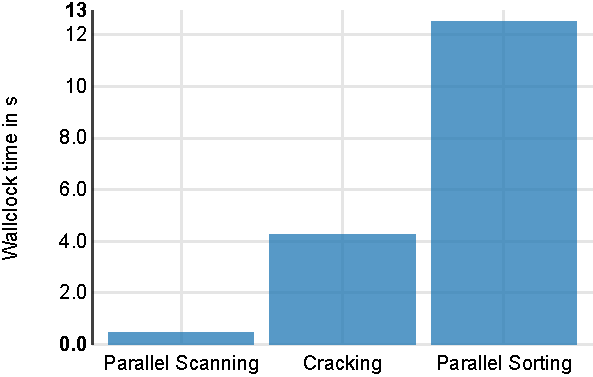
\includegraphics[width=.9\columnwidth]{Figures/damon/Motivation}
  \caption{Costs of Database Operations}
\vspace{-0.2 in}
  \label{fig:motivation}
\end{figure}
%
It shows that while an off-the-shelf \emph{(Parallel) Mergesort}
implementation\footnote{Part of the GNU libstdc++ Version 4.8.2} is
about 30 times more expensive than a (quasi I/O bound) \emph{(Parallel)
  Scan}, it is only three times as expensive as MonetDB's
implementation of \emph{Cracking}~\cite{DBLP:conf/cidr/IdreosKM07}.
Even though both \emph{Scanning} and \emph{Cracking},
(sequentially) read and write the same amount of data, they have
vastly different costs. The performance difference must, thus, be
due to their computational costs: \emph{Cracking}
is, unlike \emph{Scanning}, not I/O bound. However,\\[-2ex]
\begin{center}
  \begin{minipage}{.95\linewidth}
    \emph{we believe} that, if implemented with the underlying
    hardware in mind, \emph{Cracking} can be (roughly) I/O bound.
\end{minipage}
\end{center}
\vspace{1ex}
%
%
To validate this hypothesis, we make the following contributions:
\vspace{-1ex}
\begin{itemize}
  %\setlength{\itemsep}{0pt}
  %\setlength{\parskip}{0pt}
  %\setlength{\parsep}{0pt}
\item We conduct an in-depth study of the contributing performance factors
  of the ``classic'' \emph{Cracking} implementation.
\item Based on the findings, we develop a number of optimizations
  based on ``standard'' techniques like predication, vectorization and
  manually implemented data parallelism using SIMD instructions.
\item We develop two different parallel algorithms that exploit thread
  level parallelism to make use of multiple CPU cores.
\item We rigorously evaluate all developed algorithms on a number of
  different systems ranging from low-end desktop machines to high-end
  servers.
\end{itemize}
\vspace{-1ex}

The rest of the paper is structured as follows: In
Section~\ref{sec:related-work}, we provide an overview of related work
as well as necessary background knowledge on the optimization
techniques we applied. In Section~\ref{sec:classic-cracking} we
present our analysis of the \emph{Cracking} implementation in MonetDB
discussing its problems with regard to CPU efficiency.
We present our CPU-optimized sequential \emph{Cracking} algorithms
in Section~\ref{sec:cracking-algorithms},
and our parallel implementations in Section~\ref{subsec:tlp}.
We evaluate these algorithms on a range of different
hardware platforms in Section~\ref{sec:results} and conclude in
Section~\ref{sec:conclusion}.


\section{Background \& Related Work}
\label{sec:damon_related_work} 

Before discussing the efficient
implementation of \emph{Database Cracking}, let us briefly establish
the background knowledge regarding
\begin{inparaenum}[a)]
\item some architectural traits of modern CPUs that are relevant with
respect to implementation efficiency, and
\item partial and adaptive indexing techniques that are related to our
approach.
\end{inparaenum}

\subsection*{CPU Efficiency Techniques}
\label{sec:cpu-efficiency} Advances in processor architectures and
semiconductors have improved the performance of computer systems
steadily over the years.  However, the stagnation of clock frequency
prompted the necessity for parallelization.  Thus, modern CPUs provide
several forms of parallelism, such as instruction level parallelism,
data level parallelism and thread level parallelism.


Processors achieve \emph{Instruction Level Parallelism (ILP)} by
overlapping the execution of multiple instructions in a single clock
cycle \cite{DBLP:books/daglib/0068852}.  Independent instructions are
executed in parallel if there are sufficient resources for all of
them.  ILP can be exploited by using multiple execution units to
execute multiple instructions simultaneously (superscalar execution),
or by executing instructions in any order that does not violate data
dependencies (out-of-order execution) or even predicting the execution
of instructions (speculative execution)
\cite{DBLP:books/daglib/0028244}.  Thus, care has to be taken to
ensure that there are sufficiently many independent instructions
\cite{wheretime, DBLP:conf/cidr/BonczZN05}.

Performance improvement can also be achieved by exploiting \emph{Data
  Level Parallelism (DLP)}. In its extreme, vector processors operate
on the input arrays using one instruction per vector operation. In
practice, most modern CPUs provide \simd{} instructions that operate
on a limited number of values (vector lengths ranging from 128 to
512 bit).

Thus, fewer instructions are fetched and executed.  However, vector
instructions usually have longer latencies and lower throughput than
their scalar counterparts. They also rely on their inputs being stored
in a contiguous (often even \simd{}-word-aligned) memory region. In
the most modern instruction sets (AVX2 and AVX-512), there is support
for gather (AVX2 \& AVX-512) and scatter (only AVX-512) instructions
that fetch data from, respectively save data to, multiple, non-contiguous memory locations.
Recent papers study the implementation of various database operations,
e.g., scans, aggregations, index operations and joins, using SIMD
instructions~\cite{database_SIMD}, while \cite{hash_join_rev,
  hash_sort_SIMD} provide a thorough analysis of hash join and
sort-merge join using SIMD.  These operations significantly benefit
from the SIMD technology by exploiting DLP and by eliminating branch
mispredictions.

\emph{Thread Level Parallelism (TLP)} allows multiple threads to work
simultaneously.  This allows an application to take advantage of TLP
by splitting into independent parts that run in parallel.  The
advantage of multithreading is even more significant in systems that
are equipped with multiple CPUs or multicore CPUs (chip
multiprocessors).  In addition, many chip multiprocessors incorporate
the hyper threading technology which increases parallelism by allowing
each physical core to appear as two logical cores in the operating
system. Heavy load components such as instruction pipelines, registers or
the execution units are usually replicated while others, such as caches,
are shared among the logical cores.  Basic database operations have
been reexamined exploiting TLP, e.g., aggregations \cite{aggr_tlp} and
join algorithms \cite{hash_join_rev,hash_sort_SIMD}.


\subsection*{Indexing Techniques}
\label{sec:indexing-techniques} In the majority of automated index
tuning approaches, index tuning is clearly distinct from query
processing.  Offline indexing approaches
\cite{DBLP:conf/vldb/AgrawalCKMNS04, DBLP:conf/vldb/DagevilleDDYZZ04,
DBLP:conf/vldb/ZilioRLLSGF04} analyze a given workload and
select/create the necessary indexes before the workload enters the
system, whereas online indexing approaches
\cite{DBLP:conf/icde/BrunoC07, DBLP:conf/icde/LuhringSSS07,
DBLP:conf/sigmod/SchnaitterAMP06} continuously monitor the workload
and periodically reevaluate the index selection.  In both cases,
indexes equally cover all data items, even if some of them are not
heavily queried.  Thus, both index tuning and index creation may
negatively affect the workload performance if there is not enough idle
time to build the indexes or/and if the workload arbitrarily changes.

Adaptive indexing \cite{ DBLP:conf/edbt/GraefeK10,
  DBLP:conf/cidr/IdreosKM07, DBLP:journals/pvldb/IdreosMKG11} is a
recent, lightweight approach to self-tuning databases: data
reorganization is integrated with query processing.  \emph{Database
  Cracking} \cite{DBLP:conf/cidr/IdreosKM07} is an implementation of
the adaptive indexing concept.  Database Cracking initializes a
partial index for an attribute the first time it is queried.  Future
queries on the same attribute further refine the index by partitioning
the data using the supplied query predicates as pivots (similar to
quicksort \cite{quicksort}) and updating the secondary dictionary
structure. Since the reorganization of the index is part of the select
operator, \emph{Database Cracking} can be seen as an alternative
implementation of scanning. While dictionary maintenance becomes the
dominant cost factor as the average partition size
decreases~\cite{CrackRepeat}, the pivoted partitioning is the most
important factor in the beginning. In this paper we focus purely on
this step of the process, disregarding dictionary maintenance or order
propagation to other columns.


\section{Classic Cracking}
\label{sec:classic-cracking}
\emph{Database Cracking} is a pleasantly simple approach to adaptive
indexing.  However, it is not trivial to implement efficiently. In this
section, we recapitulate the original \emph{Cracking} algorithm and we
examine the problems with the current implementation regarding CPU
efficiency.

\subsection*{The Algorithm}
\label{sec:algorithm}

\begin{figure}[!t]
\begin{center}
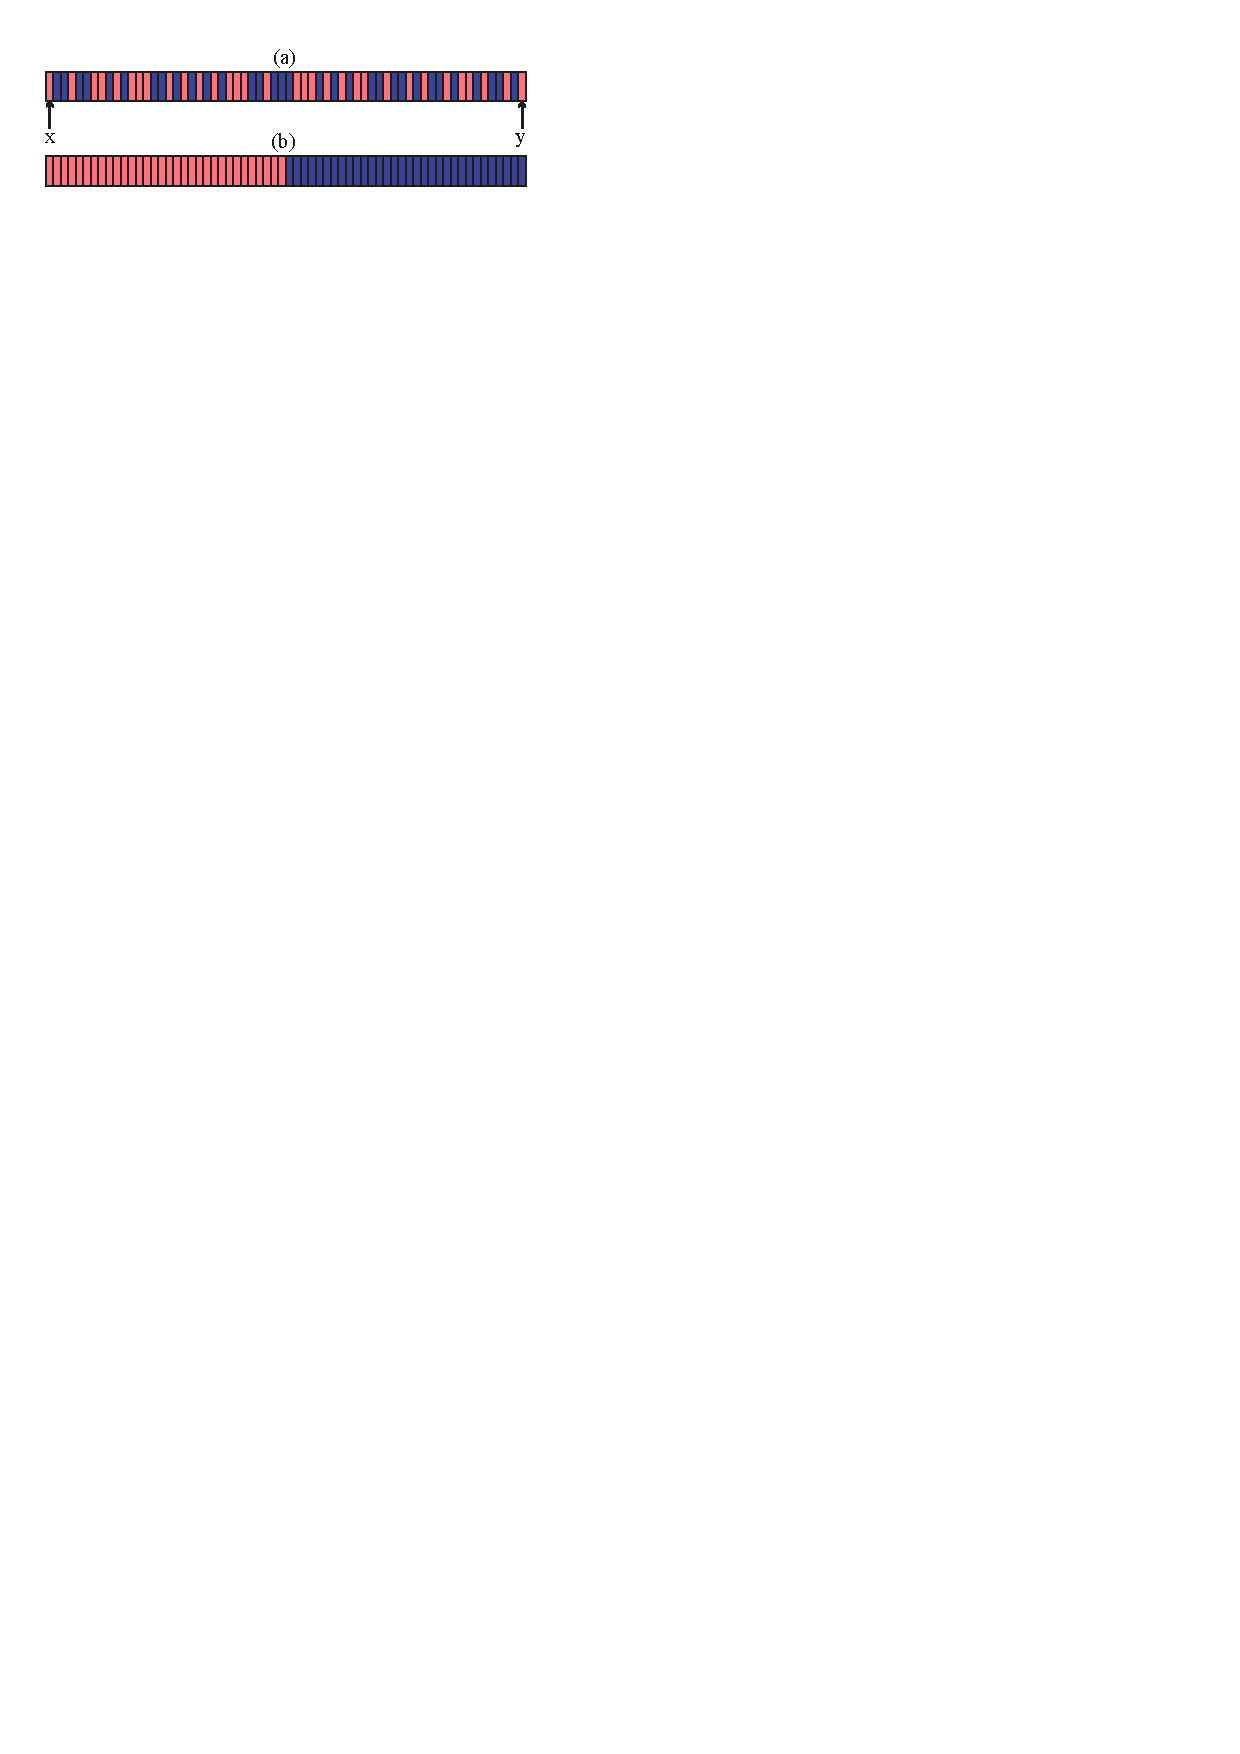
\includegraphics[trim=0.6cm 26.7cm 0cm 1cm]{Figures/damon/naive}
\vspace{-0.2 in}
\caption{Original Cracking (single-threaded)}
\vspace{-0.37 in}
\label{fig:naive}
\end{center}
\end{figure}

\begin{figure*}[t]
    \centering
  \subfloat[Cache Misses]{
    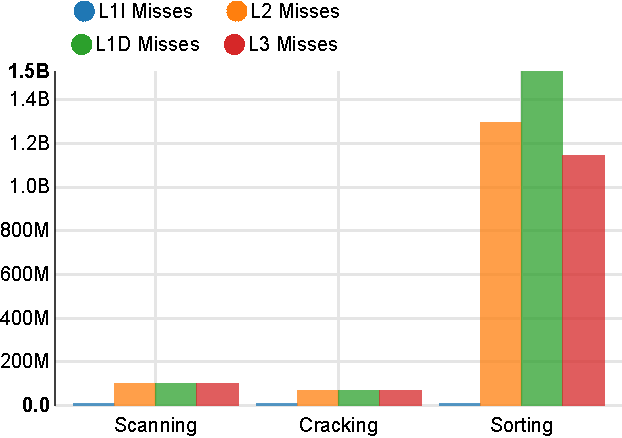
\includegraphics[width=.85\columnwidth]{Figures/damon/AnalysisCacheMisses}
\hspace{.05\columnwidth}
    \label{fig:cracking-cache-misses}
  }
  \subfloat[Costs breakdown by CPU component]{
\hspace{.05\columnwidth}
    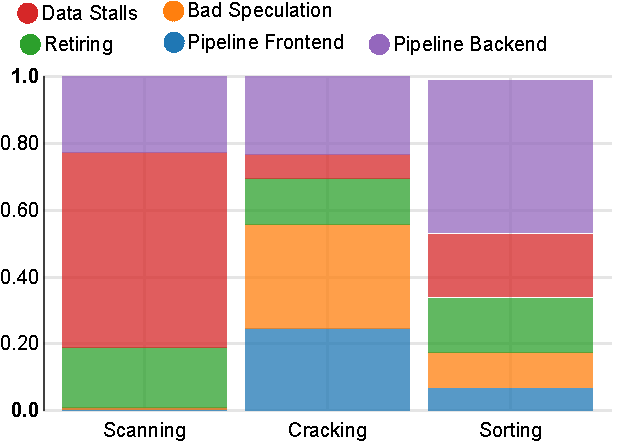
\includegraphics[width=.85\columnwidth]{Figures/damon/CostBreakdown}
    \label{fig:cracking-non-load-stalling}
  }
  \label{fig:cracking-cost-breakdown}
  \caption{Cost Breakdown of Database Operations}
\vspace{-0.2 in}
  \centering
\end{figure*}


The original, single-threaded \emph{Cracking} algorithm is illustrated
in Figure~\ref{fig:naive}.
%that is formally described in Algorithm~\ref{alg:st_cracking}.  
Figure~\ref{fig:naive}(a) depicts an uncracked piece.  Red indicates
values that are lower than the pivot, while blue indicates values that
are greater than the pivot.  Two cursors, $x$ and $y$, point at the
first and at the last position of the piece respectively.  The cursors
move towards each other, scanning the column, skipping values that are
in the correct position while swapping wrongly located values.  The
result of this process is the cracked piece shown in
Figure~\ref{fig:naive}(b).  Values that are less/greater than the
pivot finally lie in a contiguous space.  To crack a piece that
consists of $n$ values, % and a pivot in the middle.
the two cursors read all $n$ values while moving towards each other
resulting in $O(n)$ complexity in terms of computation as well as
memory access.  Thus, \emph{Cracking} and \emph{Scanning} are in the
same complexity class but have significantly different costs (recall
Figure~\ref{fig:motivation}).


\subsection*{Analysis}
\label{sec:analysis}
The classic way of analyzing in-memory data management system
performance is to count the number of cache misses at different
levels. This stems from the assumption that data management
performance is dominated by data access costs. However, as displayed
in Figure~\ref{fig:cracking-cache-misses}, the number of cache misses
do not provide an explanation for the performance difference of
\emph{Cracking} and scanning. In fact, scanning induces more cache
misses because it produces the result set out of place. This indicates
that merely looking at the number of cache misses is not sufficient -
we have to determine the costs induced in other components of the CPU.

To do so, we conducted a systematic analysis of the costs component
according to the Intel optimization manual for our (Ivy Bridge)
CPU~\cite{intelOptimizationManual}. The breakdown in Figure~\ref{fig:cracking-non-load-stalling} shows that
\emph{Cracking} merely spends 7\% of the cycles stalling because of
data access latencies. This explains why the number of cache misses
alone is a poor predictor for the overall performance. The other cost
factors, however give a much better explanation of the performance
difference between \emph{Cracking} and scanning~\footnote{In this
  normalized plot, equal height bars indicate an absolute difference of
  almost factor 10, Figure~\ref{fig:motivation} providing the scale}:
The breakdown shows that 14\% of the cycles~\footnote{or, more
  accurately microop execution slots} are spent retiring (useful)
instructions at the end of the execution pipeline. Assuming that all
instructions are necessary, this indicates that \emph{Cracking} spends
almost 10 times as much CPU cycles as scanning doing actual work. It
also gives us an upper bound on the performance that can be achieved
using a single CPU core: 14\% of the current runtime, i.e., a speedup
factor of about 7. Most importantly, however, this breakdown indicates
where there is most potential for performance improvement: in
eliminating branch mispredictions which
\begin{inparaenum}
\item cause a significant amount of wasted cycles due to \emph{bad speculation} and
\item prevent instructions from entering the \emph{pipeline} at the
  \emph{frontend}.
\end{inparaenum}



\section{CPU Efficient Cracking}
\label{sec:cracking-algorithms}
Based on the outcome of our analysis in the previous section, we can
direct our efforts to the performance painpoints of the original
\emph{Cracking} implementation, starting with branch mispredictions.

\subsection*{Predication}
\label{sec:predication}
A common technique to address costs for branch mispredictions is
``predication''. The idea is to unconditionally write output but only
advance one of the output cursors by the value of the evaluation of
the predicate. This decouples the writing operation from the predicate
evaluation and, therefore, effectively eliminates the conditional
branch instructions at the costs of more write instructions. Since
these write instructions generally only operate in L1 cache, the
performance benefit for, e.g., selections, can be
significant~\cite{ross2004selection}.
\begin{figure}[h]
\subfloat[Consistent State]{
  \includegraphics[width=.9\columnwidth]{Figures/damon/PredicationPhase1}
\label{fig:predicated-consistent}
}

\subfloat[Compare \& Write Phase]{
  \includegraphics[width=.9\columnwidth]{Figures/damon/PredicationPhase2}
\label{fig:predicated-compare-and-write}
}

\subfloat[Advance Cursor Phase]{
  \includegraphics[width=.9\columnwidth]{Figures/damon/PredicationPhase3}
\label{fig:predicated-advance-cursor}
}

\subfloat[Backup Phase]{
  \includegraphics[width=.9\columnwidth]{Figures/damon/PredicationPhase4}
\label{fig:predicated-backup}
}
  \caption{Predicated Cracking}
  \label{fig:predicated-cracking}
\end{figure}


Unfortunately, not all algorithms are equally amenable to
optimization through predication: implementations of out-of-place
algorithms like selections can speculatively write to the output
buffer as long as they write to empty slots. In-place algorithms,
however, have to ensure that they do not overwrite any of the data
values. They, therefore have to create backup copies of values
that are speculatively overwritten. Naturally, deciding which value
to backup has to be branch-free as well.

To achieve this, we developed a branch-free cracking implementation
based on predication (illustrated in
Figure~\ref{fig:predicated-cracking}). The fundamental idea is to
create a backup copy of the value that is speculatively overwritten in
a ``backup'' slot (we term the slot containing the value that is
currently processed ``active''). Based on this idea, each iteration
goes through multiple phases with all (significant) operations within
a phase being independent. At the beginning of each iteration, the
to-be-cracked array is in a ``consistent'' state (see
Figure~\ref{fig:predicated-consistent}), i.e., each input value is
stored exactly once in the array\footnote{Note that this does not
  imply that there cannot be duplicate values in the input} and the
``active'' and ``backup'' slots contain the values at both cursors.
In the \emph{Compare \& Write Phase} (see
Figure~\ref{fig:predicated-compare-and-write}), the ``active'' value
is written to both cursors and (independently) compared to the
pivot. The result of the comparison ($cmp$) is used in the next phase
(see Figure~\ref{fig:predicated-advance-cursor}) to advance the output
cursors. One cursor is advanced by the value of $cmp$, the other by
$1-cmp$. This ensures that only one of the cursors is advanced. In the
last phase (see Figure~\ref{fig:predicated-cracking}), the value at
the advanced cursor is backed up. To ensure a branch-free
implementation, we, again, use arithmetic calculations rather than
branching to select the right value to store. At the end of each
iteration, the \emph{backup} and \emph{active} slots switch roles (not
shown in figure).


We implemented this idea in two variants that vary in the way they
create the necessary backup copies of input values. The first
implementation creates the backup copies to a small (cache-resident)
buffer. This implementation has a slight disadvantage: the
compiler can either use multiple registers to hold the two slots of
the local buffer or flush the registers to L1-cache after each
phase. To alleviate this problem, we developed a variant that uses one
64-bit register to hold the ``active'' as well as the ``backup''
value. This yields a slight performance benefit~(see
Section~\ref{sec:results}).


\begin{figure}
  \centering
  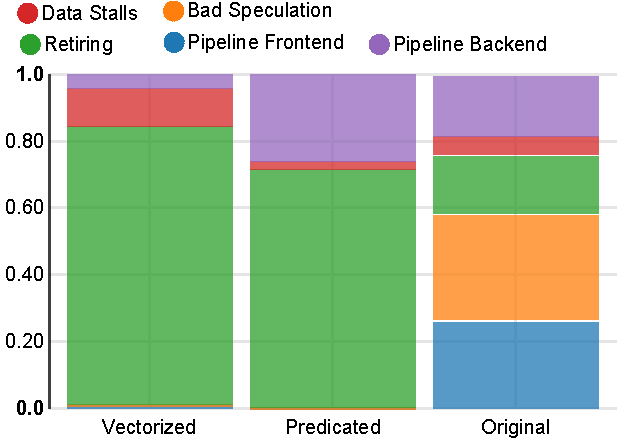
\includegraphics[width=.85\columnwidth]{Figures/damon/CostBreakdownEfficient}
  \caption{Cost breakdown of single-threaded implementations}
\vspace{-2.5ex}
  \label{fig:breakdown-efficient}
\end{figure}
\subsection*{Vectorization}
\label{sec:vectorization}
The main problem with the predicated implementation is the effort
spent on backing up data (indicated by the \emph{Pipeline Backend} bar
which includes costs for writing data in
Figure~\ref{fig:breakdown-efficient}).  The main tuning parameter for
this operation is the granularity at which data is copied. Naturally,
copying larger chunks results in more predictable code (at
compile-time as well as run-time). The extreme case for this
optimization would be copying the entire input-array, making it an
out-of-place implementation. This is not only memory intensive but
also cache-inefficient since it requires two scans of the data. The
natural solution to this problem is vectorization: small,
cache-resident chunks of the input data are copied and, subsequently,
partitioned out-of-place (see
Figure~\ref{fig:vectorized-cracking}). This has the advantage of
producing tight, CPU-efficient loops in the (expensive) partitioning
phase while allowing bulk-backups of input values.

However, the lack of control in the partitioning phase slightly
complicates things in the backup: we have to deal with overflowing
output buffers. It is, therefore, not enough to back up one vector per
side since a half-full buffer may overflow into the adjacent one. This
requires additional backup slots to ensure that the distance between
each read-cursor and the trailing write-cursor is greater than the
size of a vector. As visualized in
Figure~\ref{fig:vectorized-cracking}, three backup slots are
sufficient to maintain enough ``slack space'' for safe writing.

\subsection*{SIMD}
\label{subsec:single-threaded-simd}
Figure~\ref{fig:breakdown-efficient} indicates that more than 80\% of
the cycles of the cracking implementation are now spent retiring
(useful) instructions. This indicates that, to further improve
single-threaded performance, we have to perform more work per
instruction. This can be achieved by the use of SIMD instructions. The
AVX-2 instruction set of current Intel CPUs provides instructions to
gather values from multiple addresses into an SIMD word in a single
instruction. The opposite, i.e. scatter instructions, are, however,
only available in AVX-512 which is, currently, only supported by the
Intel Xeon Phi extension cards. We, therefore, implemented
\emph{Cracking} using AVX-2 instructions to gather the input
values. The main idea is to have one cursor per SIMD lane, gathering
values that satisfy the partitioning predicate until the word is
filled and can be flushed. We implemented all necessary operations
(comparison, cursor advancing, ...)  using 256-bit SIMD instructions
and predication.

During evaluation~(see Section~\ref{sec:results}), we found that this
algorithm generally performs worse than the previously discussed
implementations. We include the description primarily for completeness
sake.
\begin{figure}[!t]
\begin{center}
\includegraphics[trim=0cm 24.5cm 0cm 1cm,width=2.3\columnwidth]{Figures/damon/vectorized}
\vspace{0ex}
\caption{Vectorized Cracking}
\vspace{-2.5ex}
% \vspace{-0.26 in}
\label{fig:vectorized-cracking}
\end{center}
\end{figure}

\section{Parallelization}
\label{subsec:tlp}

In this section we present two \emph{Cracking} algorithms that exploit thread-level parallelism, i.e.,
first a simple partition \& merge parallel algorithm, and 
then a refined variant of the simple algorithm.

\subsection*{Partition \& Merge}
\label{subsubsec:partition-merge}

\begin{figure}[!t]
\begin{center}
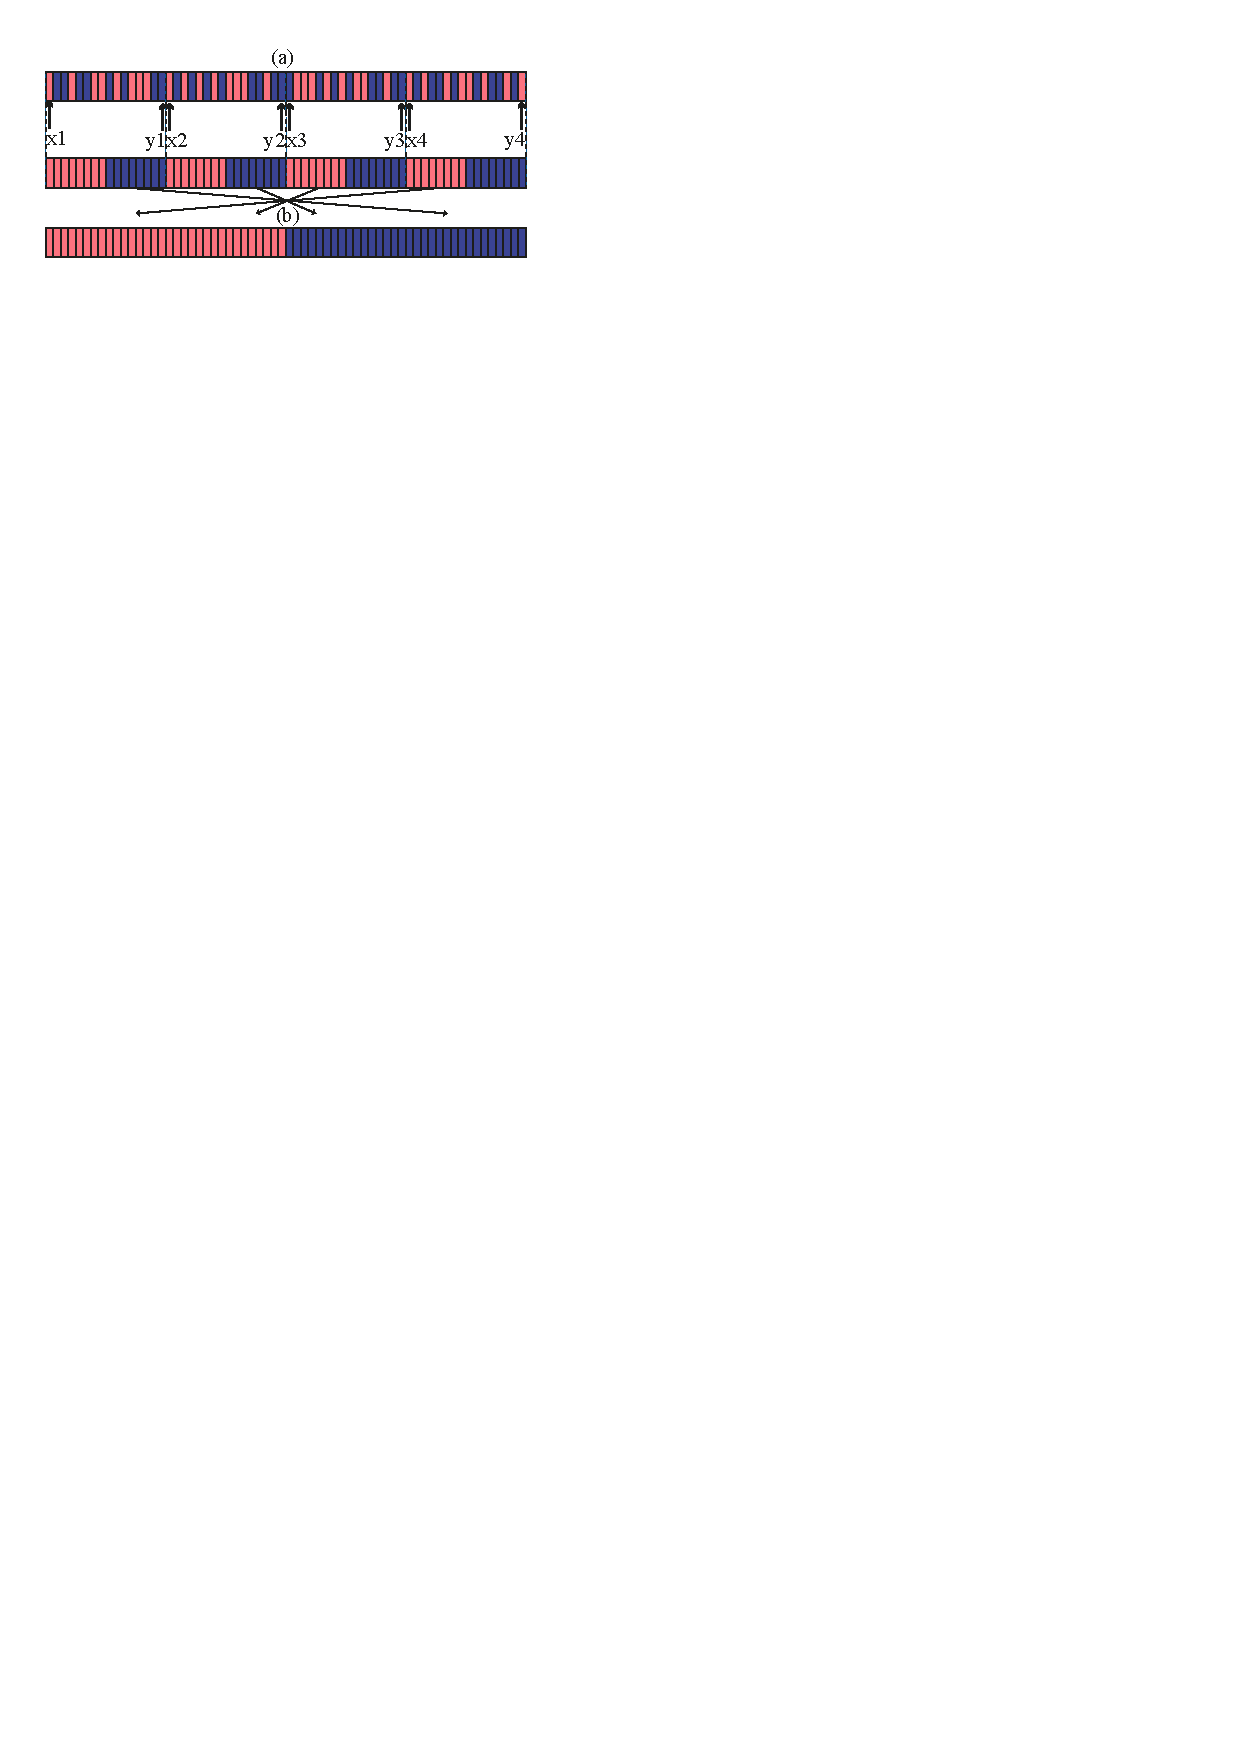
\includegraphics[trim=0.6cm 25.5cm 0cm 1cm]{Figures/damon/mcrack1}
% \vspace{-0.1 in}
\caption{Simple Partition \& Merge (multi-threaded)}
\vspace{-2.5ex}
% \vspace{-0.1 in}
\label{fig:mcrack1}
\end{center}
\end{figure}

The simple parallel \emph{Cracking} algorithm divides an
uncracked piece into $T$ consecutive partitions that are
concurrently cracked by $T$ threads.  Each thread cracks a partition by
applying the original \emph{Cracking} algorithm.  Finally, during the merge phase, a single thread swaps
wrongly located blocks of values into their final position.
Figure~\ref{fig:mcrack1} shows an instance of the simple parallel
\emph{Cracking}.  Four threads crack four partitions concurrently.
Red indicates values that are less than the pivot, while
blue indicates values that are greater than the pivot.  
After cracking all partitions, the merge phase takes place, i.e., a single thread relocates blocks of elements to the correct positions, resulting in the final cracked piece shown in Figure~\ref{fig:mcrack1}(b).
During the merge phase the relocation of data causes many cache misses, which can be avoided with the refined partition \& merge \emph{Cracking} described in the following subsection.

\subsection*{Refined Partition \& Merge}
\label{subsubsec:refined-partition-merge}

\begin{figure}[!t]
\begin{center}
\includegraphics[trim=0.6cm 25.7cm 0cm 1cm]{Figures/damon/mcrack2}
% \vspace{-0.2 in}
\caption{Refined Partition \& Merge (multi-threaded)}
\vspace{-2.5ex}
% \vspace{-0.4 in}
\label{fig:mcrack2}
\end{center}
\end{figure}
The refined partition \& merge \emph{Cracking} algorithm divides the uncracked
piece into $T$ partitions.  
The center partition is consecutive with
size $S=\#elements/\#threads$, while the remaining $T-1$ partitions consist of two disjoint
pieces that are arranged concentrically around the center partition.
Assuming the selectivity is known and it is expressed as a fraction of 1, the size of the left piece equals to $S*selectivity$, while the size of the right piece equals to $S*(1-selectivity)$.
For instance, in Figure~\ref{fig:mcrack2}(a), the size of the disjoint pieces is equal, since the selectivity is 0.5 (50\%).
As in the simple partition \& merge \emph{Cracking}, $T$ threads
crack the $T$ partitions concurrently applying the original \emph{Cracking} algorithm.  
The thread that cracks the center (consecutive) partition, swaps values within this partition.
Each thread that cracks two disjoint pieces swaps wrongly located values between the
two pieces.  For example, in Figure~\ref{fig:mcrack2}(a) one thread exchanges values between the first and the last piece.
Finally, a single thread (as in the simple parallel algorithm) locates wrongly-located blocks to the correct positions.

Although the refined algorithm swaps values that are in longer
distance compared to the simple algorithm, it moves less data during
the merge phase, because more data is already in the correct position.
For instance, in Figure~\ref{fig:mcrack2} only two values are located in wrong positions, while in Figure~\ref{fig:mcrack1}, we relocate 6 blocks of 8 values each.
Both parallel algorithms make $O(n)$ comparisons/exchanges during the partitioning phase.
However, the merging cost is significantly lower for the refined partition \& merge \emph{Cracking} algorithm.  


\subsection*{CPU Efficiency \& Parallelization}

In principle, the single-threaded CPU efficiency improvements as presented in
Section~\ref{sec:cracking-algorithms} are orthogonal to the thread-level
parallelism presented above. Consequently, we can combine both techniques,
hoping to accumulate their benefits. We focus on vectorization as this proved
to yield better single-threaded CPU efficiency than predication or SIMD
(cf., Sections~\ref{sec:cracking-algorithms} and \ref{sec:results}).

Vectorization of the simple partition \& merge \emph{Cracking} algorithm is
straight-forward.  We simply have each thread perform vectorized
\emph{Cracking} instead of original \emph{Cracking} on its contiguous
partition.  With the refined partition \& merge \emph{Cracking} algorithm,
we need to additionally handle the case that, in case of skewed data, one of
the two write cursors exceeds its partition half, and thus needs to
``fast-forward'' (or ``jump'') to the other half to continue.


\section{Evaluation}
\label{sec:results}

\subsection*{Setup}
\label{sec:hardware-platforms}
We evaluated the presented implementations\footnote{Available for
  download
  at\\\mbox{\hspace{.5em}\url{http://www.cwi.nl/~holger/cracking/sortvsscan}}}
on four different machines (see Table~\ref{tab:hardware}): a
\$300-class desktop machine, a \$1,000-class workstation, a
\$10,000-class server and a \$60,000-class high-end server.  All
experiments were evaluated on an array with 5GB of 32-bit integer
values with varying selectivity/pivot position. We used Fedora 20, a
3.13.5 Linux kernel and gcc version 4.8.2. Since we compare single- as
well as multi-threaded algorithms, we measure the average unix
wallclock time of seven (memory-resident) runs rather than spent
CPU-cycles or microop execution slots.
\begin{table}[t!]
  \centering
% BEGIN RECEIVE ORGTBL hardware
\begin{tabular}{|l|l|l|l|l|}
\hline
Class & CPU & Cores & ISA & RAM \\
\hline
Desktop & AMD E-350 & 2 & SSE4a & 8GB \\
Workstation & Intel i7-4770 & 8\tablefootnote{Including virtual cores (Hyperthreading)} & AVX-2 & 32GB \\
Server & 2$\times$Intel E5-2650 & 2$\times$16$^{6}$ & AVX & 256GB \\
HE Server & 4$\times$Intel E5-4657L & 4$\times$24$^{6}$ & AVX & 1024GB \\
\hline
\end{tabular}
% END RECEIVE ORGTBL hardware
\begin{comment}
#+ORGTBL: SEND hardware orgtbl-to-latex :splice nil :skip 0
|-------------+--------------------------+-----------------------------------------------------------+-------+-------|
| Class       | CPU                      | Cores                                                     | ISA   | RAM   |
|-------------+--------------------------+-----------------------------------------------------------+-------+-------|
| Desktop     | AMD E-350                | 2                                                         | SSE4a | 8GB   |
| Workstation | Intel i7-4770            | 8\tablefootnote{Including virtual cores (Hyperthreading)} | AVX-2 | 32GB  |
| Server      | 2$\times$Intel E5-2650v2 | 2$\times$16$^{5}$                                         | AVX   | 256GB |
| Server      | 2$\times$Intel E5-2650v2 | 2$\times$16$^{5}$                                         | AVX   | 256GB |
|-------------+--------------------------+-----------------------------------------------------------+-------+-------|
\end{comment}
% | \textbf{Workstation (IB)} | \textbf{Intel i7-3770S}    | \textbf{AVX} | 16GB  |
  \caption{Hardware Setup}
\vspace{-1ex}

  \label{tab:hardware}
\end{table}


\subsection*{Results}
\label{sec:results-1}
\begin{figure}[p!]
\vspace{.4ex}
\hspace{8.8em}
\includegraphics[height=5ex]{Figures/damon/LegendLeft} 
\end{figure}
%\newcommand{\scalefactor}[0]{.78}
\begin{figure}[p!]
\centering
  \subfloat[Desktop]{
  \includegraphics[width=0.5\columnwidth]{Figures/damon/SingleThreadedPebble}
  \label{fig:single-threaded-desktop}
}

  \subfloat[Workstation]{
  \includegraphics[width=0.5\columnwidth]{Figures/damon/SingleThreadedPan}

  \label{fig:single-threaded-workstation}
}

\subfloat[Server]{
  \includegraphics[width=0.5\columnwidth]{Figures/damon/SingleThreadedBricks}
  \label{fig:single-threaded-server1}
}

\subfloat[High-End Server]{
  \includegraphics[width=0.5\columnwidth]{Figures/damon/SingleThreadedDiamonds}
  \label{fig:single-threaded-server2}
}
\caption{Single Threaded Performance}
  \label{fig:single-threaded-performance}
\end{figure}

\begin{figure}[p!]
\hspace{-2.5em}
\includegraphics[height=5ex]{Figures/damon/LegendRight} 
  % \includegraphics[width=0.309414338\textwidth]{LegendRight}  
\end{figure}

\begin{figure}[p!]
\centering
  \subfloat[Desktop]{
  \includegraphics[width=0.5\columnwidth]{Figures/damon/MultiThreadedPebble}
  \label{fig:multi-threaded-desktop}
}

  \subfloat[Workstation]{
  \includegraphics[width=0.5\columnwidth]{Figures/damon/MultiThreadedPan}

  \label{fig:multi-threaded-workstation}
}

\subfloat[Server]{
  \includegraphics[width=0.5\columnwidth]{Figures/damon/MultiThreadedBricks}
  \label{fig:multi-threaded-server1}
}

\subfloat[High-End Server]{
  \includegraphics[width=0.5\columnwidth]{Figures/damon/MultiThreadedDiamonds}
  \label{fig:multi-threaded-server2}
}
\caption{Multi Threaded Performance}
  \label{fig:multi-threaded-performance}
\end{figure}

\subsubsection*{Single-threaded Cracking}
\label{sec:single-threaded}
At first, let us look at single threaded performance
(Figure~\ref{fig:single-threaded-performance}): we are comparing the
original cracking implementation to the single-threaded predicated (in
register as well as cache) and the vectorized version. For reference,
we also include the costs for the (parallel \& predicated) scan which
is (roughly) memory access bound in most cases (large intermediates
lead to expensive swapping on the desktop). The first observation is
that (the original) \emph{Cracking} is most expensive at 50\%
selectivity (incidentally the most useful case when considering the
indexing aspect of \emph{Cracking}). This is to be expected since this
case yields the worst branch prediction performance. We observe that,
at 50\% selectivity, all systems benefit significantly from
predication. Beyond that, things become more complicated. While the
server and workstation systems achieve a benefit from keeping
``active'' and ``backup'' values in the same register, it even has a
negative effect on the performance of the desktop system (that,
surprisingly, decreases with increasing selectivity). While the
branch-free algorithms perform better than the original
\emph{Cracking} for most of the selectivity spectrum, the better CPU
performance does not outweigh the additional writes towards the ends
of the spectrum. This is a common observation with predicated
algorithms that stems from the better branch prediction at the ends of
the spectrum.


\subsubsection*{SIMD}
\label{sec:simd}
One of the most interesting (and disappointing) results of our
experiments is the performance of the SIMD-based \emph{Cracking}
implementation (see Figure~\ref{fig:simd-performance}). The figure
shows that the SIMD implementation performs significantly worse than
the best single-threaded implementation (Vectorized) on our
workstation system. It is even outperformed by the original
\emph{Cracking} implementation. While surprising at first, modeling
the costs of this implementation provides a satisfying explanation:
since an SIMD-word is only flushed to the output when it is completely
filled with qualifying values, it (usually) takes multiple gathers to
process one SIMD-word. Since every pointer has a certain probability
to read a qualifying value, filling the SIMD-word can be modeled as a
binomial process. The average number of gathers per flush can be
derived from this model using stochastic analysis (we omit the details
for lack of space). For a word-length of 8 values and a pivot in the
middle of the range, it takes around 4.42 gathers to fill a
word. Given that each gather costs 6 cycles (on Nehalem), it takes, on
average, more than three cycles per value to only gather the
values. Adding the costs for cursor advancing and predicate
evaluation, the costs of the SIMD-implementation are prohibitively
high.
\begin{figure}
  \centering
  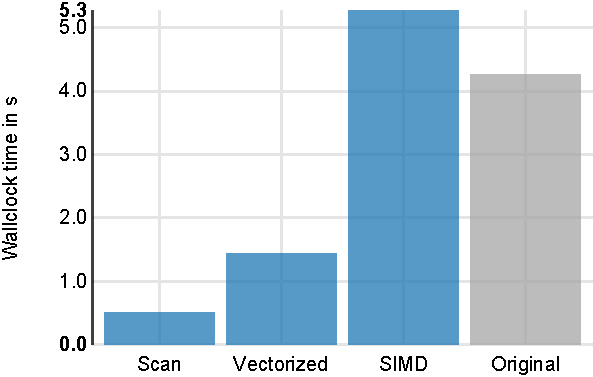
\includegraphics[width=.7\columnwidth]{Figures/damon/SingleThreadedSIMD}
  \caption{SIMD Processing Performance at 50\% Selectivity}
\vspace{-1ex}
  \label{fig:simd-performance}
\end{figure}



\subsubsection*{Multi-threaded}
\label{sec:multi-threaded}
The results of our multi-threaded experiments are displayed in
Figure~\ref{fig:multi-threaded-performance}. To accommodate to the
varying number of cores in our experimentation platforms, we set the
degree of parallelism to the number of (virtual) cores in each machine
(see Table~\ref{tab:hardware}). For reference, we include the best
single-threaded implementation (Vectorized) in the chart. We observe a
significant speedup in almost all cases. Naturally, the \emph{Refined
  Partition \& Merge} implementation performs better than its plain
counterpart. In addition, both implementations achieve a performance
improvement if combined with vectorization. This effect is, however
less pronounced on the highly parallel server systems. On the 96-core
High-End Server system it is virtually non-existent. In general, we
found the \emph{Vectorized Refined Partition \& Merge} implementation
the fastest of our implementation across all parameters. In fact, it
even outperforms (parallel \& predicated) scanning in some cases: the
in-place nature of \emph{Cracking} yields fewer cache-line fill misses
than the out-of-place scan and gives it a (slight) performance edge.



\section{Summary}
\label{subsec:damon_conclusion}
\emph{CPU-efficient implementation of even simple algorithms is hard}:
while common knowledge in many fields of computer science, this
insight is still not properly appreciated in the field of data
management. In this paper, we conducted an in-depth study of such a
supposedly simple algorithm: pivoted partitioning. We demonstrated
that, in its na\"ive implementation, it is not an I/O bound
algorithm. Starting from this understanding, we systematically
analyzed and addressed the dominant cost factors using
state-of-the-art techniques. The result is in an implementation that
rivals and sometimes even outperforms a parallelized scan on a variety of
systems. In that, it is up to 25 times faster than the initial


\clearpage

%-----------HOLISTIC INDEXING--------------
\input{Chapters/holistic/hol}
\section{Introduction}
\label{sec:intro}

\begin{table*}
\begin{center}

\begin{tabular}{ccccccc}
\hline
\cline{1-7}
Indexing& Statistical&Exploitation of idle resources & Exploitation of idle resources & Index  		 & Updates, & Workload\\
        & analysis   & \emph{before} query processing& \emph{during} query processing & materialization  & projection cost &\\
\hline
Offline & $\surd$ & $\surd$ & $\times$  & full & high & static \\ 
Online & $\surd$ & $\times$ & $\surd$  & full & high & dynamic\\
Adaptive & $\times$ & $\times$ & $\times$  & partial & low & dynamic\\
Holistic & $\surd$ & $\surd$ & $\surd$  & partial & low & dynamic\\
\hline
\label{tab:qualitative}
\end{tabular}
\vspace{-0.45cm}
 \caption{Qualitative difference among offline, online, adaptive and holistic indexing.}
\vspace{-0.7cm}
\end{center}
\end{table*}

The big data era is causing the research community to rethink fundamental issues 
in the design of database systems  
towards more usable systems \cite{UsableDatabases} that can access data better and faster 
%\cite{blinkdb,MAD,shark,exploration,hinge, hazy,earl,GuidedInteraction, RequirementsSciDB, datacuration,energypartitioning},
\cite{exploration,hinge, hazy,earl},
 that can better exploit modern hardware and opportunities for massive parallelization
%\cite{swissbox,elastras,hadoop+,cod,dbseer},
\cite{hadoop+}
 that can support efficient processing of OLTP and/or OLAP queries
% \cite{nodb,shareddb,hstore,hyper,bitweaving}
 \cite{nodb,hstore,hyper,bitweaving}.
% or even exploit crowdsourcing for query processing \cite{crowdq,crowddb}.

\textbf{The Physical Design Problem.} 
Physical design, and in particular proper index selection, is a predominant factor for the performance of database systems and has only become more crucial in the big data era.
With new dynamic and exploratory environments, physical design becomes especially hard given the instability of workloads and the continuous stream of big data; a single physical design choice is not necessarily correct or useful for long stretches of time, while at the same time workload knowledge is scarce given the exploratory user behavior.

\textbf{State-of-the-Art.} In database applications, where ``the future is known'', physical design is assigned to database administrators
who may also be assisted by auto-tuning tools 
\cite{DBLP:conf/vldb/AgrawalCKMNS04,DBLP:conf/vldb/DagevilleDDYZZ04,DBLP:conf/vldb/ZilioRLLSGF04}.
Still though, a significant amount of human intervention is necessary and everything needs to happen offline.
Thus, offline indexing can be applied with good results only on applications where there is enough workload 
knowledge and idle time to prepare the physical design appropriately before queries arrive.

Unfortunately, for many modern applications ``the future is unknown'', e.g., in scientific databases, social networks, web logs, etc.
In particular, the query processing patterns follow an exploratory behavior, which changes so arbitrarily that it cannot be predicted.
Such environments cannot be handled by offline indexing.
Online indexing \cite{DBLP:conf/icde/BrunoC07,DBLP:conf/sigmod/SchnaitterAMP06} 
and adaptive indexing \cite{DBLP:conf/cidr/IdreosKM07} 
are two approaches to automatic physical design in such dynamic environments, but none of them in isolation handles the problem sufficiently.
Online indexing periodically refines the physical design but it may negatively affect running queries every time
it needs to use resources for reconsidering the physical design and it may not be quick to follow the workload changes as it reacts only periodically. 
Adaptive indexing does not have this problem as it introduces continuous, incremental and partial index refinement 
but it adjusts the physical design only during query processing based on queries.

\textbf{Always Indexing.}
In this paper, we make the observation that in real systems there are plenty of resources that remain under-utilized and 
we propose to exploit those resources to be able to better address dynamic and  ad-hoc environments. 
In particular, we focus on exploiting CPU cycles to the maximum by continuously detecting idle CPU cycles
and using them to refine the physical design (in parallel with query processing).
Such idle CPU cycles occur when the system  does not exploit all available cores up to 100\%.
% (non-peak workload).
%i.e., either because the workload is not enough to saturate the CPUs or because the current tasks performed for 
%query processing are not easy to parallelize to the point where all available CPU power can be  exploited
%or when there are no active user queries (\emph{idle time}).
We distinguish between ``\emph{idle time}'' as in
``\emph{there is no user-driven workload at all and the entire CPU (all its hardware contexts) is idle (except possible occasional operating system background activity)}''
and ``\emph{idle CPU resources}'' as in
``\emph{the active user-driven workload does / can not use all physically available CPU hardware contexts.}'' 
Intuitively, there are two options when resources are under-utilized but still there are active queries in the system.
The first option is to introduce more parallel query processing algorithms to maximize utilization for the existing workload. The second one is to exploit the extra resources towards a different goal (extra indexing actions in our case). We investigate and compare both directions.


%\begin{figure}[t]
%\begin{center}
%\includegraphics[trim=4cm 22cm 12cm 2.8cm]{qualitative}
%\caption{Indexing Approaches.}
%\vspace{-0.4 in}
%\label{fig:various}
%\end{center}
%\end{figure}

\textbf{Holistic Indexing.} In this paper, we introduce a new indexing approach, 
called \emph{holistic indexing}.
Holistic indexing  addresses the automatic physical design problem in 
modern applications with  dynamic and exploratory workloads.
%\textcolor{red}{where there is no prior knowledge about how many under-utilized CPU resources will be available}.  
It continuously monitors the workload and the CPU utilization; 
when idle CPU cycles are detected, holistic indexing exploits them in order to partially and incrementally 
adjust the physical design based on the collected statistical information.
Each index refinement step may take only a few microseconds to complete and the system will typically perform
several such steps in one go depending on available system resources.
Everything happens in parallel to query processing but without disturbing running queries.
The net effect is that holistic indexing refines the physical design,
% there are more chances for future queries to enjoy better  data access patterns.
improving performance and robustness by enabling better data access patterns for future queries.
Table~\ref{tab:qualitative} summarizes the qualitative difference between holistic indexing and current state-of-the-art indexing approaches.
Compared to past approaches, holistic indexing manages to minimize both initialization and maintenance costs, 
as it relies on partial indexing, and to exploit all possible CPU resources
%before and/or during query processing, 
in order to provide a more complete physical design.

\textbf{Contributions.}
Our contributions are as follows:
\vspace{-0.5em}
\begin{itemize}
  \setlength{\itemsep}{0pt}
  \setlength{\parskip}{0pt}
  \setlength{\parsep}{0pt}
\item We introduce the idea of exploiting idle CPU resources towards 
continuously adapting the physical design to ad-hoc and dynamic workloads.
\item We discuss  in detail the design of holistic indexing on top of modern column-store architectures, i.e.,
how to detect and exploit idle CPU resources during query processing.
\item We implemented holistic indexing in  an open-source column-store, MonetDB \cite{DBLP:journals/debu/IdreosGNMMK12, monetdb}.
%\textcolor{red}{The code is publicly available in \cite{holindex}.} 
Through a detailed experimental analysis both with microbenchmarks and with TPC-H 
we demonstrate that we can exploit idle CPU resources to prepare the physical design better,
leading to significant improvements over past indexing approaches in dynamic environments. 
\end{itemize}
\vspace{-0.5em}

\textbf{Paper Structure.} The rest of the paper is structured as follows:
Section~\ref{sec:relwork} provides an overview of related work.
In Section~\ref{sec:background}, we shortly recap the basics of column-store architectures 
and the basics of adaptive indexing.
Then, Section~\ref{sec:problem} introduces holistic indexing, while Section~\ref{sec:experiments} presents a detailed experimental analysis.
Finally, Section~\ref{sec:conclusions} discusses future work and concludes the paper. 



\section{Holistic Indexing}
\label{sec:problem}

In this section we discuss the fundamentals of holistic indexing.
We designed holistic indexing on top of column-store architectures inspired by their flexibility on manipulating some attributes without affecting the rest.
During query processing indices are built and optimized incrementally by adapting to query predicates, as in adaptive indexing.
However, in contrast to adaptive indexing, index refinement actions are not triggered only as a side-effect of query processing; 
in holistic indexing incremental index optimization actions take place continuously in order to exploit 
under-utilized CPU cores. Thus, concurrently with user queries, system queries also refine the index space.
Holistic indexing monitors the workload and CPU resources utilization and every time it detects that the system is under-utilized
it exploits statistical information to decide which indices to refine and by how much. 

Thus, with holistic indexing we achieve an always active 
self-organizing DBMS by continuously adjusting the physical design to workload demands.

\vspace{2mm}
\emph{\textbf{Problem Definition:} Given a set of adaptive indices, statistical information about the past workload, storage constraints and the CPU utilization, continuously select indices from the index space and incrementally refine them, while the materialized index space size does not exceed the storage budget.}
\vspace{2mm}

In the rest of this section, we discuss in detail how we fit holistic indexing in a modern DBMS architecture. 

\subsection{Preliminary Definitions}
\label{subsec:definitions}

First, we give a series of definitions.

\textbf{Workload.} A workload \emph{W} consists of a sequence of user queries, inserts and deletes. Updates are translated into a deletion that is followed by an insertion.

\textbf{CPU Utilization.} CPU utilization in a time interval $dt$ describes how much of the available CPU power is used in $dt$. Specifically, it expresses the percentage of total CPU time, i.e., the amount of time for which the CPU is used for processing user or kernel processes instead of being idle. CPU utilization is calculated using (operating system) kernel statistics.

\textbf{Configuration.} A configuration is defined as a set of adaptive indices that can be used in the physical design.
There are three kinds of configurations.
The \emph{actual configuration}, \emph{C$_{actual}$}, contains indices on attributes that have already been accessed by user queries in the workload.
Indices are inserted in \emph{C$_{actual}$} when they are created during query processing.
For instance, assume a query $Q$ enters the system and contains a selection on an attribute $A$.
If the adaptive index on $A$ does not exist, it is created on-the-fly and it is inserted in \emph{C$_{actual}$}.

Besides \emph{C$_{actual}$}, holistic indexing also maintains the \emph{potential configuration}. \emph{C$_{potential}$},
 which contains indices on attributes that have not been queried yet.
Indices are inserted in \emph{C$_{potential}$} either automatically by the system or manually by the user.
Finally, the \emph{optimal configuration}, \emph{C$_{optimal}$}, contains indices that have reached the optimal status (the next paragraph describes when an index is considered optimal).
The union of \emph{C$_{actual}$} and \emph{C$_{potential}$} constitutes the index space \emph{IS}, i.e., the indices which are candidates for
incremental optimization when the system is under-utilized.
Later, in Section~\ref{subsec:design}, we describe how the system is educated to pick an index from \emph{IS}.
Indices from \emph{C$_{optimal}$} are not considered for further refinement during the physical design reorganization.

\textbf{Optimal Index.} 
Holistic indexing exploits adaptive indices.
As seen in Section~\ref{subsec:cracking}, an adaptive index is refined during query 
processing by physically reorganizing pieces of the cracker column based on query predicates.
As more queries arrive, more pieces are created, and thus, the pieces become smaller.
We have found that when the size of the pieces becomes equal to L$_{1}$ cache size ($|L_1|$), further refinements are not necessary;
a smaller size increases administration costs to maintain the extra pieces and it does not bring any significant extra benefit as scanning inside L$_{1}$ is fast anyway (no cache misses).
Pieces of size smaller than L$_{1}$ cache can either be sorted 
or queries simply need to scan them (a range select operator has to scan at most two L$_{1}$ pieces).
An index \emph{I} on an attribute $A$ is considered optimal (\emph{I$_{opt}$}), 
when the average size of pieces ($|p|$) in $A_{CRK}$ is equal to the size of L$_{1}$ cache.
Equation \eqref{eq:d} describes the distance between \emph{I} and \emph{I$_{opt}$}.
\vspace{-0.25em}
\begin{equation}
d(I,I_{opt}) = |p| -|L_{1}| = \frac{N_A}{p_A} - |L_{1}|
\label{eq:d}
\vspace{-0.25em}
\end{equation}

$N_A$ is the total number of tuples in $A_{CRK}$ while $p_A$ is the total number of pieces in $A_{CRK}$.
This information is readily available and thus we can easily calculate the average piece size
in a cracker column and in turn we can calculate the distance of the respective cracker index from its optimal status.

\textbf{Statistical Information.} 
During query processing holistic indexing continuously monitors the workload and the CPU utilization.
For each column in the schema it collects information regarding how many times it has been accessed by user queries,
how many pieces the relevant cracker column contains, how many queries did not need to further refine the index
because there was an exact hit.
Besides the statistical information about the workload, kernel statistics are used in order to monitor the CPU utilization.


%\newpage
\subsection{System Design}
\label{subsec:design}

Holistic indexing is always active.
It continuously monitors the workload and the CPU utilization.
When under-utilized CPU cores are detected, holistic indexing exploits them in order to adjust the physical design based
on the collected statistical information.
The system performs several index refinement steps simultaneously depending on available CPU resources. 
Everything happens in parallel to query processing, but without disturbing running queries.


We discuss in detail the continuous tuning process and how to exploit under-utilized CPU cycles. We also discuss how existing adaptive indexing solutions on %
 core database architectures issues%
 such as updates and concurrency control can be directly adapted to work with holistic indexing.


\textbf{Statistics per Column/Index.}
Statistics per column are collected during query processing.
This is the job of the select operator as it is within the select operator that all (user query) 
adaptive indexing actions take place.  
Every time an attribute is accessed for a selection of a user query, the select operator
updates a data structure, which contains all statistics for the respective index.
Given that the select operator performs adaptive indexing actions anyway,
it already has access to critical information such as how many new pieces were created 
during new cracking actions for this query,
whether the select was an exact match, etc.
All information is stored in a heap structure (one node per index) 
which allows us to easily put new indices in the configuration or drop old ones.
The structure is protected with read/write latches as multiple queries  or holistic workers (discussed later on) 
may be cracking in parallel.


\textbf{Tuning Cycle.} 
At all times there is an active \emph{holistic indexing thread} which runs in parallel to user queries.
The responsibility of the holistic indexing thread is to monitor the CPU utilization and to activate \emph{holistic worker threads} 
to perform auxiliary index refinement actions whenever idle CPU cycles are detected.
The tuning process is shown in Figure~\ref{fig:diagram}.
The holistic indexing thread continuously monitors the CPU load at intervals of  $1$ second at a time.
In case holistic worker threads are activated, the holistic indexing thread waits for all worker threads to finish and measures the CPU utilization within the next $1$ second. 
In our analysis, we found that $1$ second is the time limit that gives proper kernel statistics.
%In addition, while the worker threads are activated, we do not measure the CPU utilization in order to avoid including the CPU power consumed by the worker threads. 
When $n$ idle CPU cores are detected, $n$ holistic worker threads are activated.
Each worker thread executes an instance of the IdleFunction, which picks an index from the Index Space $IS$ and performs $x$ 
partial index refinement actions on it.
Every time an index is refined, the respective statistics, e.g., distance from the optimal index, are updated.
When an index reaches the optimal status, it is moved into the optimal configuration \emph{C$_{optimal}$}.

A side-effect of the tuning process is that some of the holistic worker threads might remain idle while the holistic indexing thread waits for all workers to finish.
However, as we show later in Section~\ref{subsec:motivation} (Figure~\ref{fig:motiv}(d)), this happens only for very short periods of time and as 
the system adapts to the workload this phenomenon disappears (as the pieces queried in the adaptive indices become smaller and smaller 
the holistic indexing workers end up doing tasks of similar weight as none is going to touch a very big piece).


\textbf{Index Refinement.}
Every time a worker thread wakes up, it performs $x$ index refinements on a single column. $x$ is a tuning parameter. 
In our analysis in Section~\ref{subsec:decisions} (Figure~\ref{fig:cracks_number}) we found that a good value for our hardware set-up is $x=16$. 
The index refinements are performed by picking $x$ random values in the domain of the respective
attribute and cracking the column based on these values. In this way, each time a worker thread cracks a single
piece of a column it splits this piece into two new pieces based on the pivot. 

There are numerous choices on how to choose a pivot. We found that picking a random pivot is the most cost efficient choice.
Other options include to crack the biggest piece of the column, i.e., with the rationale that this takes more work out of future queries.
Another option is to crack the smallest piece, i.e., with the rationale that this piece is small because it is hot (because many queries access it for cracking).
However, such options are hard to achieve in a lightweight way as we need to maintain a structure such as  a priority queue
to know which piece is the biggest or smallest every time. 
Since every cracking action costs a few microseconds or milliseconds it is not worth the extra storage and CPU cost to maintain auxiliary structures.
Random pivots converge quickly to cracking the whole domain,
providing a column which is balanced in terms of which pieces are cracked
and requiring no extra costs in deciding which pivot to choose. 


\begin{figure}
\begin{center}
\includegraphics[trim=1.3cm 18.5cm 0cm 2.7cm]{Figures/holistic/diagram}
\vspace{-0.6 in}
\caption{Tuning actions.}
\vspace{-0.7 cm}
\label{fig:diagram}
\end{center}
\end{figure}

\textbf{Index Decision Strategies.} 
Another decision we have to make is which index to refine out of the pool of candidate indices.
Here, we describe four different strategies we can follow in order to pick an index from the index space.
The notion behind the first three strategies is that, since the only information we have is the past workload, 
we can exploit this information in order to prepare the physical design for a similar future workload.
On the contrary, the fourth strategy makes random choices.

For all strategies, a weight \emph{W$_{I}$} is assigned to each index \emph{I} in the index space.
When an index \emph{I} is added in the candidate indices, its weight is initialized 
to the distance between \emph{I} and \emph{I$_{opt}$}, which is given by Equation \eqref{eq:d}. 
For each index $I$, initially, there is only one partition (p$_{I}=1$) in \emph{I}, i.e., the entire column. 
Thus, the initial weight \emph{W$_{I_{init}}$} is equal to $N_{I} - L_{1_{s}}$,
where $N_{I}$ is the cardinality of the respective attribute (with type $T$) and $L_{1_{s}}$ is the number of elements of type $T$ that can fit into $L_{1}$ cache. 
The weight is used as a priority number in the first three strategies.
The index with the highest priority, i.e., the maximum weight,  in \emph{C$_{actual}$} is refined first.
When \emph{W$_{I}$} becomes equal to zero, \emph{I} is transferred 
from \emph{C$_{actual}$} to \emph{C$_{optimal}$} and it is not considered for further refinement in the future.
If \emph{C$_{actual}$} is empty, an index is randomly picked from \emph{C$_{potential}$}.
The weight of each index is constantly updated after every index refinement regardless of whether it is caused
by a user query or by holistic indexing.
Below we describe the four strategies.

\vspace{-0.2cm}
\begin{itemize}
  \setlength{\itemsep}{0cm}
  \setlength{\parskip}{0cm}
  \setlength{\parsep}{0cm}
\item \textbf{W1:} $W_{I}=d_{I}=d(I,$$I_{opt})$. Using this strategy, we give a priority to indices with large partitions.  
\item \textbf{W2:} $W_{I}=f_{I}*d_{I}$. Priority is given to indices that have large partitions and at the same time are accessed frequently in the workload. $f_{I}$ is the number of user queries that access $I$.
\item \textbf{W3:} $W_{I}=(f_{I}-f_{I_{h}})*d_{I}$. In this strategy we try to identify indices that are accessed frequently in the workload and at the same time have large partitions, because they have a high hit rate. These indices have a smaller priority compared to indices with large partitions that are accessed less frequently. $f_{I}$ is the number of user queries that access $I$, while $f_{I_{h}}$ is the number of user queries that do not trigger a refinement of $I$ because the requested value bound already exists in $I$.
\item \textbf{W4:} Make a random choice.
\end{itemize}
\vspace{-0.2cm}

Overall, our analysis, which is described later in Section~\ref{subsec:strategies} (Figure~\ref{fig:hvsc}), with numerous workloads showed
that even though small improvements can be achieved when picking the perfect strategy for each workload,
the random strategy gives a good and robust overall solution that is always close to the best for all workloads.
 
\begin{figure}
%\begin{center}
\hspace{3em}
\includegraphics[trim=2.5cm 13cm 1.5cm 2.5cm,width=0.4\textwidth]{Figures/holistic/latching}
\vspace{0.5em}
\caption{Concurrency control in holistic indexing.}
\vspace{-0.4cm}
\label{fig:conc}
%\end{center}
\end{figure}
%\newpage
\textbf{Concurrency Control.}  
An index refinement due to holistic indexing happens in parallel with user queries.
Since user queries may also cause refinement of adaptive indices, we need to properly control
these changes. In addition, as more than one holistic thread may be active at any time, they may 
be trying to refine the same index. 
The study of concurrency control for adaptive indexing \cite{DBLP:journals/pvldb/GraefeHIKM12, DBLP:journals/vldb/GraefeHIKMS14} showed that it is possible to allow multiple
concurrent index refinements in adaptive indices via lightweight concurrency control, i.e., relying only on latches of individual pieces
in an adaptive index.
The point is that an index refinement only changes the structure of the index and not its contents (contrary to an actual update).
In this case, an index refinement only rearranges values in a single piece of a column at a time.
Thus it is sufficient to allow
other queries to work on different pieces in parallel by taking 
read/write latches on individual pieces, called piece latches in \cite{DBLP:journals/pvldb/GraefeHIKM12, DBLP:journals/vldb/GraefeHIKMS14}.
We exploit these techniques here in order to allow user queries and holistic workers to work concurrently over a single column, but
we also identify extra opportunities to increase parallelism for holistic workers.

Figure~\ref{fig:conc} shows an example of an adaptive index where two queries are actively cracking it.
Each query is interested in its own value range and needs to crack one piece, i.e., at the value of its selection.
The idea is that \emph{all} other pieces of the column are available for index refinement by holistic worker threads.
One direction would be that each holistic worker decides which piece of an index to refine
by picking from a list of pieces that currently have no locks.
However, such information is expensive to maintain similarly to our discussion in the ``Index Refinement'' paragraph.
Thus, holistic workers make random choices regarding which value to use as pivot and thus which piece to crack.
However, when a holistic worker requests a write latch to crack a piece and it happens that the piece is locked at the moment, then 
if the latch is not given immediately, the worker picks another random pivot and repeats the procedure
until it finds a free piece to crack. In contrast, user queries need to always block in such cases and wait for the piece to be unlocked.
For instance, in Figure~\ref{fig:conc}(d) the holistic worker thread tries to lock piece 2.1, which is already locked by Q4.
Instead of waiting for the lock to be released, the worker chooses another pivot.
The new pivot falls in piece 3.2, which is not locked and it is reorganized finally by the worker (Figure~\ref{fig:conc}(e)).
As we process more queries and as we perform more holistic indexing, 
the number of pieces in an index grows; as a side-effect 
the waiting time for taking a latch decreases as there are more candidate pieces to pick from.


\textbf{Updates.} 
Updates for adaptive indexing have been studied in \cite{DBLP:conf/sigmod/IdreosKM09}.
The design in \cite{DBLP:conf/sigmod/IdreosKM09} is that updates remain as pending updates
and are merged during query processing, i.e., if a query requests a value range that contains one or more pending updates,
then only those updates are merged on-the-fly and without destroying any of the information on the adaptive index.
Each query needs to lock at most one column piece at a time for cracking and can update this piece at the same time if pending updates for this piece exist \cite{DBLP:journals/pvldb/GraefeHIKM12, DBLP:journals/vldb/GraefeHIKMS14}. Multiple queries may work in parallel updating and cracking separate pieces (value ranges) of the same column.

The difference here is that with holistic indexing, holistic workers not only perform
auxiliary index refinement actions but also merge pending updates.
That is, if a holistic worker picks a pivot which falls within a piece of the respective column and the value range,
for which this piece holds values, has pending updates, then all those pending updates are merged by the holistic worker.
In this way, holistic worker threads not only refine the adaptive indices in the background but also bring them 
more up to date which removes further load from future queries.

\begin{figure}[!t]
\begin{center}
\includegraphics[trim=-0.5cm 25.7cm 0.5cm 1cm,width=2\columnwidth, height=1.8cm]{Figures/holistic/mcrack2}
\vspace{-0.25 in}
\caption{Refined Partition \& Merge (multi-threaded) \cite{efficient_cracking}.}
\vspace{-0.7cm}
\label{fig:mt-cracking}
\end{center}
\end{figure}

\begin{figure}[!t]
\begin{center}
\includegraphics[trim=0cm 24.5cm 0cm 1cm,width=2.3\columnwidth,height=2.8cm]{Figures/holistic/vectorized}
\caption{Vectorized Cracking \cite{efficient_cracking}.}
\label{fig:vectorized-cracking}
\vspace{-0.7cm}
\end{center}
\end{figure}

\begin{figure*}[!t]
     \begin{center}
	 \subfloat[Performance]{%
	\includegraphics[trim=2cm 2.2cm 15cm 21.7cm]{Figures/holistic/motivation}
	}%
	 \subfloat[Performance Breakdown]{%
	\includegraphics[trim=2.3cm 2.1cm 15cm 21.7cm]{Figures/holistic/hist_motivation}
	}%
	 \subfloat[Index Partitions]{%
	\includegraphics[trim=2.3cm 2.2cm 15cm 21.7cm]{Figures/holistic/pieces_motivation}
	}%
	 \subfloat[Idle CPU Utilization]{%
	\includegraphics[trim=2cm 2.2cm 15.5cm 21.7cm]{Figures/holistic/workers}
	}%
	\vspace{-0.25 in}
	\caption{Improving performance with holistic indexing.}
	\vspace{-0.7 cm}
	\label{fig:motiv}
     \end{center}%\end{figure*}
\end{figure*}

\textbf{Storage Constraints.} 
Holistic indexing works within a limited storage budget.
Adaptive indices may be dropped or recreated at any time. 
They consist auxiliary information and thus dropping an index does not lead to any loss of data.
In case the storage budget does not allow adding a new index triggered by a user query, 
then indices are removed with a least frequently used (LFU) policy from the index space
at an index-level granularity or at a fine-grained granularity that allows for creating and dropping individual ranges dynamically, as partial cracking suggested in \cite{DBLP:conf/sigmod/IdreosKM09}.

\textbf{Multi-core Adaptive Indexing.}
The goal of holistic indexing is to improve the physical design by fully utilizing the available CPU resources.
An alternative approach to achieve maximum CPU utilization is to parallelize the index refinement actions triggered by user queries.
This problem was studied in \cite{efficient_cracking}, which introduced a multi-core, CPU efficient cracking algorithm shown in Figure~\ref{fig:mt-cracking}.
In this algorithm, the to-be-cracked piece is partitioned initially into as many slices as the number of threads, e.g., $n$ (Figure~\ref{fig:mt-cracking}(a)).
The center slice is contiguous, while the
remaining $n-1$ slices consist of two disjoint halves, each, that are arranged
concentrically around the center slice ($x_{i}$ and $y_{i}$ indicate the first and the last element of piece $i$ respectively).
$n$ threads crack the $n$ slices independently applying a vectorized, out-of-place cracking algorithm (Figure~\ref{fig:vectorized-cracking}), which was proven  in 
\cite{efficient_cracking} to be the most CPU efficient single-threaded cracking implementation reported so far.
Finally, the local data are merged into a big cracked piece (Figure~\ref{fig:mt-cracking}(b)).
We found that devoting all resources to perform adaptive indexing for user queries in parallel does not lead to the absolute best performance. 
Specifically, we found that we can improve performance even more by assigning part of the resources to holistic indexing. 
In this way, some of the CPU resources are assigned to parallel cracking for user queries but the rest of the CPU resources
are distributed across several holistic workers for additional index refinements.
In the experimental section we show why this approach is better than assigning all available resources to user queries.



\section{Experimental Analysis}
\label{sec:experiments}

In this section, we demonstrate that holistic indexing leads to a self-organizing always-on DBMS
with substantial benefits in terms of response time; with zero administration or set-up effort
holistic indexing improves performance adaptively by exploiting all available CPU resources to the maximum.
We present a detailed experimental analysis using both standard benchmarks such as TPC-H and
real-life workloads such as SkyServer as well as synthetic microbenchmarks for a fine-grained analysis.

We use a dual-socket machine equipped with two 2.00 GHz Intel(R) Xeon(R) CPU E5-2650 processors and with 256 GB RAM.
Each processor has 8 hyper-threading cores resulting in 32 hardware threads in total.
The operating system is Fedora 20 (kernel version 3.12.10).
All experiments we report are based on an implementation of holistic indexing in MonetDB 
%\textcolor{red}{\cite{holindex}} 
and assume a main-memory environment.

\subsection{Improving over State-of-the-Art Indexing}
\label{subsec:motivation}

In our first  experiment we demonstrate that holistic indexing 
has the potential to bring substantial performance improvements over existing state-of-the-art indexing approaches.
We test holistic indexing against parallel versions of adaptive indexing (database cracking), 
offline indexing, online indexing and plain scans.

For plain scans (no indexing), we use a parallel select operator implemented in MonetDB.
For offline and online indexing we sort the columns using a highly parallel NUMA-aware sorting algorithm that was introduced in \cite{hash_join_rev} (m-way, 16-byte keys) and is publicly available in \cite{psort_site}.
Specifically, in offline indexing we pre-sort all the columns before query processing, while in online indexing we assume that after processing a few queries we understand the workload patterns and then we sort the relevant columns.
MonetDB automatically detects that a column is sorted and can use efficient binary search actions during select operations.
For adaptive indexing we use the parallel vectorized database cracking algorithm that was introduced in \cite{efficient_cracking} (see Section~\ref{subsec:design}).
%Initially, the input attribute is distributed across NUMA regions.
%Each thread locally sorts the respective NUMA-local chunk applying scalar sorting (qsort).
%Finally, local sorted chunks are merged into a globally sorted copy of the attribute.

  
Here we use a synthetic benchmark.
The query workload consists of 10$^{3}$ range select queries over a table of  10 attributes;
each query touches a single attribute  (we will see more complex queries later on).
Each attribute consists of 2$^{30}$ uniformly distributed integers,
while the value range requested by each query (and thus the selectivity) is random. 
All queries are of the following form.

\vspace{0.5em}
\centerline{\emph{select A from R where A < v}}
\vspace{0.5em}

The tested scenario assumes a dynamic and ad-hoc environment 
with zero workload knowledge and zero idle time to pre-index the data. 
Figure~\ref{fig:motiv}(a)  shows the results.
On the \emph{x}-axis queries are ranked in execution order.
The \emph{y}-axis represents the cumulative response time as the query sequence evolves, 
i.e., each point $(x, y)$ represents the sum of the execution time $y$ for the first $x$ queries.
In this way, the graph shows how the response times evolve as we process more and more queries.

If there is no indexing support (plain scans), the entire column/ attribute is scanned in parallel by 32 threads for every query.
Because of this stable access pattern, the cumulative response time of the query sequence grows linearly
as every query has similar cost.
With offline indexing, on the other hand, it takes 12 seconds to completely sort each column, assuming a priori workload knowledge.
This leads to a 120 seconds initialization overhead to sort all 10 columns.
Since there is no idle time before the first query, the sorting cost is added to the execution time of the very first query in Figure~\ref{fig:motiv}(a).
After the first query, all queries are answered with fast binary search actions which results in a rather flat cumulative curve.
With online indexing, the first 100 queries are answered without any index support and thus the cost grows linearly.
After the 100th query,  assuming enough workload knowledge has been obtained via monitoring, we proceed to sort all 10 columns.
The sorting cost is added to the execution cost of the 101st query, since there is no idle time between the 100th and the 101st query.
As with offline indexing, all subsequent queries are answered extremely fast with binary search over the sorted column.
Nevertheless, both in offline and in online indexing, the whole query sequence is affected by the sorting costs.
On the other hand, adaptive indexing continuously improves performance requiring no workload knowledge 
and without penalizing individual queries. This improvement comes from the fact that adaptive indexing builds only partial indices
which it incrementally refines as queries arrive.
However, there is still room for big improvements.


\begin{figure}
\begin{center}
\includegraphics[trim=1.8cm 2cm 0cm 22.3cm]{Figures/holistic/thread_distribution}
\vspace{-0.2 in}
\caption{Performance improves if we distribute the threads equally between user queries and holistic workers.}
\vspace{-0.7 cm}
\label{fig:thread_distribution}
\end{center}
\end{figure}
Holistic indexing manages to further improve the performance of the workload by about 50\%.
Contrary to the other indexing approaches, 
MonetDB with holistic indexing enabled monitors the CPU utilization and constantly  tries to maximize it.
When holistic indexing detects idle CPU resources, it triggers index refinement actions on existing adaptive indices.
In this experiment, an index is inserted in the index set, and specifically in $C_{actual}$, when a user query creates it.
For holistic indexing the actual user queries behave in exactly the same way as in adaptive indexing, i.e., the first
query will create an adaptive index and subsequent queries refine it using the very efficient and almost linearly
scaling parallel vectorized cracking implementation from \cite{efficient_cracking}.
The difference is that with holistic indexing enabled idle CPU resources are exploited towards further refining the adaptive indices
in a way which does not hurt running queries.
Since parallel vectorized cracking \cite{efficient_cracking} is designed to be CPU efficient, encountering only very little resource stalls,
we generated kind of a worst-case scenario for holistic indexing: we limited the maximal
number of hardware context assigned to user queries to 16 (equal to number
of physical cores), leaving at least 16 (otherwise not effectively usable
by the prime user query workload) hardware contexts (``hyper-threads'')
available for holistic indexing.
Constantly, our load-checker usually detects 16 idle hardware contexts, and consequently
starts 8 holistic indexing workers (each using two threads) as shown in
Figure~\ref{fig:motiv}(d). Figure~\ref{fig:thread_distribution} shows that the combination of using maximal 16 (out of
32) hardware contexts for user queries (performing parallel vectorized adaptive indexing \cite{efficient_cracking}), while devoting any
remaining idle hardware context to holistic indexing, improved the overall
performance by a factor 2 over using all 32 hardware contexts for user
queries (and thus none for holistic indexing).


Figure~\ref{fig:motiv}(b) is a breakdown 
of the performance of holistic indexing and adaptive indexing.
The \emph{y}-axis represents the total response time of the first query, the next 9 queries, etc.
The total height of each bar represents the total response time to run the entire workload of $10^3$ queries.
The first few queries do not see any improvement because holistic indexing cannot concurrently refine a column if there are user queries cracking it. 
This is because initially columns have not been 
cracked at all and thus the first few user queries will lock big pieces for cracking. However,
as each column is cracked into smaller pieces, holistic indexing may invoke  actions to refine 
a column even if concurrent queries are cracking it. 
Essentially, each user query needs to lock at most one piece of an adaptive index at a time, i.e., the piece it is about to crack,
and thus holistic indexing may choose any of the remaining pieces to perform further index refinements.

Holistic indexing outperforms adaptive indexing by a factor 2 by injecting additional index refinements on top of those that adaptive indexing does anyway.
Figure~\ref{fig:motiv}(c) shows the amount of pieces which have been created in all 10 adaptive indices; holistic 
indexing creates more pieces than adaptive indexing. 
As a result, 
future
\begin{wrapfigure}{l}{0.166\textwidth}
\begin{center}
\includegraphics[trim=2.9cm 2cm 18.5cm 23.7cm]{Figures/holistic/cost_graph}
\vspace{-0.1in}   %-0.1in
\caption{\small{Adaptive Ind.}}
\vspace{-0.7cm}
\label{fig:cost_graph}
\end{center}
\end{wrapfigure}
 user queries need to touch less data as they find a fine-grained index, and thus performance improves for holistic indexing. As Figure~\ref{fig:cost_graph}
 shows, the first queries that access the same index run slower, because they reorganize big partitions. Thus, additional
pieces have to be inserted in the index as early as possible in the query sequence.


As discussed in Section~\ref{subsec:design}, on some occasions 
the main holistic indexing thread waits for all workers to finish before assigning new tasks,
leaving under-utilized CPU resources for some brief periods. 
Figure~\ref{fig:motiv}(d) shows how the total response time 
of all workers in every tuning cycle changes over time and as the  query sequence evolves.
The right $y$-axis shows the number of holistic worker threads the holistic indexing thread activates whenever it detects idle CPU resources.
The maximum number of workers that holistic indexing can activate is 8. %, i.e., equal to the number of cores in our system.
The left $y$-axis represents the total response time of all workers during a single tuning cycle. 
The $x$-axis represents the activations  of holistic indexing.
A single activation of holistic indexing triggers the activation of multiple holistic workers.
The total response time of the workload is 90 seconds.
Within this amount of time, holistic indexing is activated only 15 times, because of the waiting time (1 second) between two CPU load measurements and because of the waiting time until all workers finish in every tuning cycle.
We observe that the response time of the workers is high only for the first few activations and reduces very fast as the index becomes fine-grained. In this way, the system adapts on its own and eventually no worker is a bottleneck.

Holistic indexing sees even bigger performance benefits when there is idle time before query processing.
When there is idle time and no workload knowledge, holistic indexing chooses random indexes to insert in $C_{potential}$  and refines them until the first query arrives. Here using the same set-up as in the previous experiment, we manually induce idle time and holistic indexing adds 10 random indices in $C_{potential}$ .
Figure~\ref{fig:apriori} shows the results.
Compared to adaptive indexing, which does not exploit the a priori idle time
\begin{wrapfigure}{l}{0.166\textwidth}
\begin{center}
\includegraphics[trim=2.8cm 1.8cm 18cm 23cm]{Figures/holistic/hist_motivation_apriori}
\vspace{-0.2in}
\caption{Indexing.}
\vspace{-0.7cm}
\label{fig:apriori}
\end{center}
\end{wrapfigure}
e (22 seconds), holistic indexing exploits 
this time to spread tuning actions over 10 indices.
Thus, when user queries are processed they reorganize smaller partitions and the benefit is already obvious in the beginning of the workload compared to Figure~\ref{fig:motiv}(b), where the benefit in the workload appears after the 10th query when all indices have been inserted in the index set automatically by the system.

By being able to completely automatically utilize available CPU resources and direct them 
towards lightweight actions that may improve future requests,
holistic indexing can bring significant performance gains on top of existing indexing approaches. 
It outperforms adaptive indexing by a factor 2 in terms of individual query performance
At the same time it outperforms offline and online indexing, especially in the beginning of the workload, 
when offline indexing penalizes the first queries with the index building cost and online indexing does not provide any indexing support
until the 100th query.
Besides the difference in performance, the qualitative difference described in Table~\ref{tab:qualitative}, makes holistic indexing a very appealing indexing approach in modern dynamic environments.

%\vspace{-0.2 in}

\begin{figure*}[t]
     \begin{center}

        \subfloat[Random]{%
            \label{fig:random_pred}
            \includegraphics[trim=2cm 2cm 16.3cm 24cm]{Figures/holistic/random_predicates}
        }%
	\subfloat[Skewed]{%
            \label{fig:skew_pred}
            \includegraphics[trim=2cm 2cm 16.3cm 24cm]{Figures/holistic/skew_predicates}
        }%
      \subfloat[Periodic]{%
           \label{fig:periodic_pred}
           \includegraphics[trim=2cm 2cm 16.3cm 24cm]{Figures/holistic/periodic_predicates}
        }%
       \subfloat[Sequential]{%
            \label{fig:sequential_pred}
            \includegraphics[trim=2cm 2cm 16.3cm 24cm]{Figures/holistic/sequential_predicates}
        }%
       \subfloat[SkyServer]{%
            \label{fig:sequential_pred}
            \includegraphics[trim=2cm 2cm 16.3cm 24cm]{Figures/holistic/skyserver_predicates}
        }%
\vspace{-0.25 in}
    \caption{Various workload patterns.}
\vspace{-0.7 cm}
   \label{fig:rob1}
    \end{center}
\end{figure*}

\begin{figure}[!htb]
\begin{center}
\includegraphics[trim=1.8cm 2cm 0cm 22.4cm]{Figures/holistic/multicore}
\vspace{-0.25 in}
\caption{Holistic indexing utilizes resources more effectively than multi-core state-of-the-art adaptive indexing baselines.}
\vspace{-0.7 cm}
\label{fig:multicore}
\end{center}
\end{figure}


\subsection{Holistic Vs. Multi-core Adaptive Indexing}
\label{subsec:multicore}

Assuming there are  several CPU cores available in a modern system, 
in holistic indexing we utilize them by spreading auxiliary tuning actions across multiple indices.
An alternative way to ``keep the CPU busy'', is to parallelize the existing adaptive indexing algorithms.
In this experiment we study how state-of-the-art adaptive indexing baselines compare to holistic indexing. In particular, we study parallel vectorized database cracking (PVDC), parallel vectorized stochastic database cracking (PVSDC) \cite{efficient_cracking} and a modified version of parallel chunked coarse granular index (P-CCGI) \cite{multicore_adaptive} that we name mP-CCGI.

Stochastic cracking aims to provide robustness by performing auxiliary stochastic indexing actions.
Although stochastic cracking studied the option of collecting statistics to target the proper value ranges to index, 
it was shown in \cite{DBLP:journals/pvldb/HalimIKY12} that reacting immediately to workload changes by auxiliary 
stochastic cracking actions has a better effect (i.e., more robust).
This is because in stochastic cracking a running query performs auxiliary random cracking only within the piece that is already about to be cracked
within a given column and as a result any action brings a benefit as it imposes more order. Holistic indexing considers a much more broad space of statistics
keeping track of column-statistics to decide which columns to fine tune. 

Both stochastic cracking and plain database cracking in this experiment utilize 
multi-cores as described in the last paragraph of Section~\ref{sec:problem}.
The original P-CCGI algorithm partitions the data into as many chunks as the available number of threads and 
the first query cracks each chunk in parallel having a separate cracking index for each chunk.
Subsequent queries crack the chunks in parallel, while they benefit from the initial range partitioning.
However, this way, data that belongs in a single value range is physically stored in separate chunks/arrays 
and feeding from there other relational operators is not compatible with a column-store such as MonetDB  that relies on bulk processing;
it does not allow to exploit tight for loops without intermediate if statements to detect when we should skip from one chunk to the next during an operator. 
To address this we extended the original P-CCGI algorithm \cite{multicore_adaptive} with the ability to consolidate selection results in a single array
using the same techniques that were used for hybrid adaptive indexing which also operates on multiple chunks (but not in parallel) 
\cite{DBLP:journals/pvldb/IdreosMKG11}; each query
consolidates only the qualifying value ranges and each value range needs to be written to the contiguous array by a single query only, 
i.e., subsequent queries will only have to do consolidation if they need a new value range never consolidated before.
In a vectorized column-store this could be done without consolidation, potentially improving performance further
as has been indicated by partial sideways cracking \cite{DBLP:conf/sigmod/IdreosKM09};
vectorized processing for adaptive indexing is an open topic, though, orthogonal to this work.

The workload in this experiment consists of 10$^{3}$ select-project queries (as in the previous experiment) on 10 integer attributes.
Each attribute consists of 2$^{30}$ uniformly distributed integers.
The value range requested by each query is random while we vary
the number of available CPU cores from 2 to 32, i.e., the maximum number of cores in our system.
For holistic indexing we give half of the cores to user queries  and the rest of the cores are used by the workers (after testing all possible configurations, we found that this is the one that performs best in all cases).
The labels on top of the bars that represent the performance of holistic indexing indicate the distribution of the threads between user queries and workers in every case
(similar to Figure~\ref{fig:thread_distribution}).




Figure~\ref{fig:multicore} shows the results.
In all cases, the performance improves as we invoke more cores into query processing.
For multi-core database cracking and stochastic cracking the performance improves because many threads crack in parallel for one query at a time
while for holistic indexing performance improves because many threads work in the background in parallel with query processing
to further refine the various indices with auxiliary indexing actions.
Holistic indexing sees a bigger improvement, because it is active all the time, i.e., maximizing CPU usage.%every time it drops.
 On the contrary, multi-core vectorized database cracking and multi-core stochastic cracking improve the performance only during user queries and only during the cracking actions.
Another subtle difference but one with a major performance impact is that while stochastic cracking and database cracking target all their adaptive indexing
 actions on specific pieces as they are driven by individual queries, holistic indexing spreads its actions across the whole range of the
domain and thus across the whole range of an adaptive index (stochastic cracking does random actions but only within a single piece). 
This creates a nicely balanced index which has more potential to benefit future queries.
The modified version of P-CCGI initially range partitions the data, which can be seen as a pre-index step. 
However, this is a cost that penalizes the first set of queries.


\begin{figure}[!htb]
\begin{center}
\includegraphics[trim=1.8cm 2cm 0cm 22.8cm]{Figures/holistic/sev_workloads}
\vspace{-0.25 in}
\caption{Holistic indexing is robust.}
\vspace{-0.7 cm}
\label{fig:stochastic}
\end{center}
\end{figure}


\begin{figure*}[ht]
     \begin{center}

        \subfloat[Random Attributes - Random Values]{%
            \label{fig:random_ma}
            \includegraphics[trim=1.8cm 2.2cm 11cm 23cm]{Figures/holistic/random_ma}
        }\vspace{-0.1 in}%
	\subfloat[Random Attributes - Periodic Values]{%
            \label{fig:random_per_ma}
            \includegraphics[trim=1.8cm 2.2cm 11cm 23cm]{Figures/holistic/random_per_ma}
        }\vspace{-0.45 in}\\%
	 \subfloat[Skewed Attributes - Random Values]{%
            \label{fig:skew_ma}
            \includegraphics[trim=1.8cm 2.2cm 11cm 22cm]{Figures/holistic/skew_ma}
        }\vspace{-0.1 in}%
	\subfloat[Skewed Attributes - Periodic Values]{%
            \label{fig:skew_per_ma}
            \includegraphics[trim=1.8cm 2.2cm 11cm 22cm]{Figures/holistic/skew_per_ma}
        }%\vspace{-0.2 in}
\vspace{-0.2 in}
   \caption{%
	More performance gains for holistic indexing as more attributes exist in a schema. All strategies have similar performance.
     }%
\vspace{-0.7 cm}
    \label{fig:hvsc}
    \end{center}
\end{figure*}

\subsection{Robustness}
\label{subsec:robustness}

In our next experiment we study how holistic indexing compares to parallel database cracking and parallel stochastic cracking
in terms of robustness.
We show that holistic indexing maintains the good properties of adaptive indexing by utilizing the available CPU resources more effectively.
Both holistic indexing and the parallel variants of adaptive indexing utilize all the available CPU cores.

We test four synthetic workloads.
Each workload consists of 10$^{3}$ queries on 10 attributes ($\sim$100 queries/attribute).
Each attribute consists of 2$^{30}$ uniformly distributed integers.
The queries follow a different pattern in each workload.
The first four subfigures in Figure~\ref{fig:rob1} depict those workload patterns. 
For each workload, the respective figure illustrates graphically 
how a sequence of queries touches the value domain of a single attribute.

Furthermore, we test holistic indexing in a real-life workload using data and queries from SkyServer \cite{SkyServer}.
SkyServer collects astronomical data  and the database can be accessed publicly by individual users and institutions.
We pose $10^4$ real user queries that have been logged by the project servers on the ``Photoobjall'' table.
The ``Photoobjall'' table consists of 1.2 Billion tuples.
All queries access the ``Ascension'' attribute and are posed in exactly the same chronological order they were logged.
The pattern the SkyServer queries follow is shown in Figure~\ref{fig:rob1}(e).

Figure~\ref{fig:stochastic} shows the results.
For each indexing method we report the total time needed to process all queries for each workload.



\textbf{Synthetic Workloads.}
In all synthetic workloads holistic indexing outperforms multi-core database cracking by a factor 2-10 depending on the workload.
Multi-core database cracking is strictly driven by query predicates, and thus, can leave large unindexed pieces to be reorganized by future queries.
For instance, in the sequential workload in Figure~\ref{fig:rob1}(d), each query cracks a column in a small piece and in a big piece, and then, a future query needs to crack the big piece again, resulting in a high cost.
Multi-core stochastic cracking solves these robustness issues by injecting one extra random cracking action for each user query in order to distribute cracking more evenly.
However, holistic indexing can materialize an even bigger advantage. This is because it is not restricted to perform auxiliary index refinement actions only during user queries but it can exploit all possible CPU cycles to refine the indices, resulting in many more actions taking place in parallel with user queries. 
Moreover, holistic indexing spreads the auxiliary index refinements across the entire value domain (by choosing random pivots) without leaving big unindexed pieces.
For example, in the skewed workload in Figure~\ref{fig:rob1}(b), both multi-core database cracking and multi-core stochastic cracking show a similar performance, because they restrict the index refinements to a small region of the domain according to user query predicates, i.e, from 800 million to $2^{30}$.
Future queries have to reorganize a big unindexed area, i.e., from 0 to 800 million; this area is already indexed in holistic indexing before the 800th query arrives.
Thus, holistic indexing prepares the physical design better for (ad-hoc) future queries.



\textbf{SkyServer.} 
The SkyServer workload in Figure~\ref{fig:rob1}(e) shows the pattern 
logged in SkyServer for queries using the ``right ascension'' attribute of the ``Photoobjall'' table.
We observe that the queries follow non-random patterns, i.e., they focus on a specific part of the sky before moving to a different part.
Figure~\ref{fig:stochastic} shows that holistic indexing manages to significantly outperform multi-core database cracking 
by inducing auxiliary index refinement actions in parallel with query processing without penalizing individual user queries.

Overall, in all workloads tested, holistic indexing not only maintains the nice properties of the parallel variants of database cracking and stochastic cracking, but it also enhances the behavior further by being able to exploit
all available CPU resources effectively for a better prepared physical design.

\begin{figure*}[t]
     \begin{center}

        \subfloat[TPC-H Query 1]{%
            \label{fig:random_pred}
            \includegraphics[trim=2cm 2cm 13.5cm 22.5cm]{Figures/holistic/tpch_q1}
        }%
	\subfloat[TPC-H Query 6]{%
            \label{fig:skew_pred}
            \includegraphics[trim=3cm 2cm 15cm 22.5cm]{Figures/holistic/tpch_q6}
        }%
      \subfloat[TPC-H Query 12]{%
           \label{fig:periodic_pred}
           \includegraphics[trim=1.5cm 2cm 14cm 22.5cm]{Figures/holistic/tpch_q12}
        }%
\vspace{-0.25 in}
    \caption{TPC-H results (Scale Factor 10, ``pre-sorted'' times exclude pre-sorting costs; Q1,6,12: 8 sec).}
\vspace{-0.7 cm}
   \label{fig:tpch}
    \end{center}
\end{figure*}

%\newpage
\subsection{More Benefits with Complex Schemas}
\label{subsec:strategies}

In this experiment, we show that as the database schema becomes more complex by containing more attributes,
this brings more opportunities for holistic indexing to gain in performance;
more attributes make the indexing space bigger and thus any a priori decisions 
are even more prone to be wrong. In addition, we test the various strategies for choosing 
among the candidate indices and we show that indeed making random decisions is a robust approach. 

Here, we assume a gradually bigger database table which consists of 5-10 attributes.
Each attribute consists of $2^{30}$ uniformly distributed integers.
We fire select-project queries as in the previous experiments but this time we may query up to $X$
attributes in every run. 
Each query touches a single attribute and we vary the frequency with which each attribute is accessed, i.e.,
we run both a random workload where every attribute is evenly queried as well as a skewed workload
where some attributes are queried more than others.
For each workload we vary also the workload pattern followed by the queries.
Here, we present the results for random and periodic workload patterns.
For each case, we perform 10$^{3}$ queries.

We compare holistic indexing using one of the four strategies described in Section~\ref{subsec:design} against multi-core variants of database cracking and stochastic cracking.
Figure~\ref{fig:hvsc} shows the results;
for all cases, holistic indexing materializes a big benefit.
As the number of attributes in the database table grows, the performance benefit for holistic indexing increases. 
What happens is that holistic indexing makes sure to evenly spread
auxiliary index refinement actions across all attributes in parallel with user queries whenever free CPU
cycles are available. Then, future queries on those attributes can exploit this refined indexing. 
Compared to the case where we have a few attributes, having more attributes means that
more heavy indexing actions have to be performed overall in order to crack the columns into small pieces.
This allows holistic indexing to materialize a bigger benefit as it performs those actions in the background as opposed to 
only during user queries as in multi-core database cracking and multi-core stochastic cracking.

In addition, all index choosing strategies have similar performance on workloads where attributes are queried on random values (Figures~\ref{fig:hvsc}(a) and (c)), 
because indices are already fine-grained in such cases (even when some indices are refined more than others in a skewed workload).
However, in case of queries on periodic values (Figures~\ref{fig:hvsc}(b) and (d)) the random choice ($W4$) shows a clear performance benefit compared to the rest of the strategies, 
because it refines indices with big unindexed partitions,
and proves to be a robust design decision.


\begin{figure}[!htb]
\begin{center}
\includegraphics[trim=1.8cm 2cm 0cm 22.5cm]{Figures/holistic/cracks_number}
\vspace{-0.2 in}
\caption{Performance of holistic indexing improves while the number of index refinements $x$ increases.}
\vspace{-0.7 cm}
\label{fig:cracks_number}
\end{center}
\end{figure}


\subsection{Design Decisions}
\label{subsec:decisions}
%\vspace{-0.3cm}
\textbf{Holistic Worker Thread Refinements.}
In this experiment we demonstrate how the tuning parameter $x$, i.e., the number of index refinements per worker (Figure~\ref{fig:diagram}), affects the workload performance.
We test five workloads that consist of $10^{3}$ queries on a relation with 10 attributes as in Section~\ref{subsec:robustness} (Figure~\ref{fig:stochastic}).
We vary the number of index refinements each holistic worker thread does from 1 to 32 and we compare holistic indexing with multi-core variants of database cracking and stochastic cracking.
Figure~\ref{fig:cracks_number} shows the results.
The more index refinements each thread does, the bigger the benefit for holistic indexing because more pieces are created and thus future queries need to refine smaller pieces, touching less data.
However, when we increase the number of index refinements from 16 to 32, performance does not improve significantly, because in both cases indices converge very fast to optimal ones.
Thus, we use 16 as the number of index refinements that each holistic worker thread does in all our experiments.


\subsection{TPC-H}
\label{subsec:tpch}

In our next experiment, 
we evaluate holistic indexing on the standard database benchmark, TPC-H  \cite{tpch}.
We compare against offline indexing and relying on plain scans.
We use scale factor 10 and we test with Queries 1, 6, and 12.
For each query type, we created a sequence of 30 variations using the random query generator distributed with the benchmark. 
For offline indexing, we created the proper column-store projections by pre-sorting the data
depending on each query individually, i.e., we created the perfect projection for each query.
Specifically, for Queries 1 and 6 we created a copy of the Lineitem table sorted on the l\_shipdate attribute.
For Query 12 we created a copy of the Lineitem table sorted on the l\_receiptdate attribute.

Figure~\ref{fig:tpch} depicts the results.
For all cases, holistic indexing brings a significant advantage, resulting in a robust and stable 
performance across all queries.
The first query is slower as it creates the first adaptive indices which implies extra data copying
but after that all queries perform significantly better than plain MonetDB.
Holistic indexing matches offline  indexing without having to incur the high offline indexing cost
and without requiring any workload knowledge.
The pre-sorting cost for all queries is 8 seconds.
For Query 12, it turns out that pre-sorting does not help.
This happens because even though we may improve the selection by pre-sorting the Lineitem table,
it turns out we hurt the join between the Lineitem and the Orders table.
This is because in the base data, the Lineitem table contains 
the order date ordered and this can be exploited during the join.
With holistic indexing we do not face this problem, because the initial order changes only partially.


\subsection{Updates}
\label{subsec:updates}

So far we tested read-only workloads. 
In this experiment we demonstrate that holistic indexing maintains its nice properties  
in workloads where read-only queries interleave with write queries.
We test two scenarios.
In the first scenario (High Frequency Low Volume - HFLV), 10 inserts arrive every 10 queries.
In the second scenario (Low Frequency High Volume - LFHV), 100 inserts arrive every  100 queries.
In both scenarios the workload consists of 500 select project range queries on a single attribute $A$ and 500 insertions in total on a single attribute $A$.
While all queries are processed sequentially one after the other, the 11th query arrives 20 seconds after the 10th query resulting in idle time of 20 seconds in the system.
Attribute $A$ consists of 10$^{9}$ uniformly distributed integers.

\begin{wrapfigure}{l}{0.166\textwidth}
\begin{center}
\includegraphics[trim=2.8cm 2cm 18cm 23.2cm]{Figures/holistic/updates}
\vspace{-0.1in}   %-0.1in
\caption{Updates.}
\vspace{-0.3in}
\label{fig:updates}
\end{center}
\end{wrapfigure}
Updates are temporarily stored in a pending insertions column.
We use the Ripple algorithm \cite{DBLP:conf/sigmod/IdreosKM07} in order to apply the updates;
a pending inserted value is merged with the original data if and only if the index partition, where the specific value belongs, is refined.
Thus, the merging process happens on-the-fly and maintains the information of the index.
In this experiment we test single-threaded adaptive indexing against holistic indexing with a single worker that refines the index only during idle time.
In holistic indexing,  
auxiliary  index refinement actions also cause  insertions to be merged. In this way, holistic indexing not only refines the indices but also consumes pending
 insertions, which speeds up future queries even more and all that by exploiting idle CPU resources in parallel with query processing.
Figure~\ref{fig:updates} shows the results.
In both scenarios, holistic indexing maintains its advantage over adaptive indexing;
it is not affected by updates and still provides roughly a 50\% improvement.

%\newpage
%\vspace{-0.1cm}

\subsection{Varying Number of Clients}
\label{subsec:varcpu}

\begin{wrapfigure}{l}{0.166\textwidth}
\begin{center}
\includegraphics[trim=2cm 2cm 17cm 23cm]{Figures/holistic/threshold}
\vspace{-0.1in}
\caption{Varying number of clients.}
\vspace{-0.3in}
\label{fig:threshold}
\end{center}
\end{wrapfigure}
In this experiment we test the performance of holistic indexing with varying number of concurrent clients in the system.
Our workload consists of 1024 queries on a relation with 10 attributes.
We vary the number of concurrent clients between 1 and 32, where 32 is the number of CPU cores in our machine.
Figure~\ref{fig:threshold} shows that holistic indexing  brings a big benefit in case of a few clients.
The labels on top of the bars indicate the distribution of the available threads across user queries and holistic workers (similar  to Figure~\ref{fig:thread_distribution}).
When the number of clients increases, holistic indexing does not bring significant benefits, because it 
easily detects these cases as it monitors the CPU load continuously and so it is triggered only if the load is below a threshold.
%\newpage


%----------------------------------------------------------------------------------------
%	BIBLIOGRAPHY
%----------------------------------------------------------------------------------------

\addcontentsline{toc}{chapter}{Bibliography} 
\label{Bibliography}
\lhead{\emph{Bibliography}} % Change the page header to say "Bibliography"
\bibliographystyle{unsrtnat} % Use the "unsrtnat" BibTeX style for formatting the Bibliography
\bibliography{Bibliography} % The references (bibliography) information are stored in the file named "Bibliography.bib"
\clearpage
%----------------------------------------------------------------------------------------
%	Lists
%----------------------------------------------------------------------------------------

\lhead{\emph{List of Figures}} % Set the left side page header to "List of Figures"
\listoffigures % Write out the List of Figures
\clearpage
\lhead{\emph{List of Tables}} % Set the left side page header to "List of Tables"
\listoftables % Write out the List of Tables

%----------------------------------------------------------------------------------------
%	ABBREVIATIONS
%----------------------------------------------------------------------------------------

\clearpage % Start a new page

\setstretch{1.5} % Set the line spacing to 1.5, this makes the following tables easier to read

\lhead{\emph{Abbreviations}} % Set the left side page header to "Abbreviations"
\listofsymbols{ll} % Include a list of Abbreviations (a table of two columns)
{
\textbf{LAH} & \textbf{L}ist \textbf{A}bbreviations \textbf{H}ere \\
%\textbf{Acronym} & \textbf{W}hat (it) \textbf{S}tands \textbf{F}or \\
}

%----------------------------------------------------------------------------------------
%	SUMMARY
%----------------------------------------------------------------------------------------

\clearpage
\addcontentsline{toc}{chapter}{Summary} 
\chapter*{Summary}
\label{Summary} 

%\lhead{Chapter 2. \emph{Related Work}} % This is for the header on each page - perhaps a shortened title



\clearpage
\addcontentsline{toc}{chapter}{Samenvatting} 
\input{Chapters/Samenvatting} 

%----------------------------------------------------------------------------------------
%	ACKNOWLEDGEMENTS
%----------------------------------------------------------------------------------------
%\setstretch{1.3} % Reset the line-spacing to 1.3 for body text (if it has changed)
%\acknowledgements{\addtocontents{toc}{\vspace{1em}} % Add a gap in the Contents, for aesthetics
%The acknowledgements and the people to thank go here, don't forget to include your project advisor\ldots
%}
%\clearpage % Start a new page
\clearpage
\addcontentsline{toc}{chapter}{Acknowledgements}
\input{Chapters/Acknowledgements}

%----------------------------------------------------------------------------------------
%	SIKS
%----------------------------------------------------------------------------------------
\clearpage
\addcontentsline{toc}{chapter}{SIKS Dissertation Series}
\chapter*{SIKS Dissertation Series}
\label{siksseries}



\end{document}  
